
\section{Bottomonia production in p-p collisions: Experimental overview}


%Heavy-quark production in pp collisions provides crucial tests of our understanding
%of various aspects of QCD. The heavy-quark mass acts as a long distance cut-off
%which allows the partonic hard-scattering process to be calculated in the framework
%of perturbative QCD down to low transverse momenta ($p_T$). The formation of
%the quarkonium bound state with heavy quark pairs is non-perturbative as it involves
%long distances and soft momentum scales. Therefore, the detailed
%study of quarkonia production and the comparison to experimental data provides an
%important testing ground for both perturbative and non-perturbative aspects of QCD calculations.
 In this section, we will give an overview of measurements of $\Upsilon$
production in pp collisions at LHC and p$\overline{\rm p}$ collisions at Tevatron. 

%% Upsilon discovery

The $\Upsilon$ meson was discovered by E288 collaboration at Fermilab in the collision of
400 GeV protons with nucleus in 1977~\cite{PhysRevLett.39.252}.
%%Upsilon measurements at Tevatron
The Collider Detector at Fermilab (CDF) measured $\Upsilon$(1S), $\Upsilon$(2S) and $\Upsilon$(3S) 
differential ($d^{2}\sigma/dp_{T}dy$) and integrated cross sections in p$\overline{\rm p}$ collisions at
$\surd s$ = 1.8 TeV~\cite{CDF:1995gwi}. The three states were reconstructed via their decay 
to $\mu^{+}$ and $\mu^{-}$. The differential ($d^{2}\sigma/dp_{T}dy$) and integrated
cross sections have been measured for  $\Upsilon$(1S) and in the range
0$\textless p_{T} \textless$16 GeV/c and for $\Upsilon$(2S) and $\Upsilon$(3S)
in the range 0$\textless p_{T}\textless$10 GeV/c.
% Table~\ref{Tab:YCrossCDF95} gives $\Upsilon$ cross sections in $|y|\textless$ 0.4
%in p$\overline{\rm p}$ collisions at $\surd s$ = 1.8 TeV measured by CDF Run I with 
%luminosity of 16.6 pb$^{-1}$~\cite{CDF:1995gwi}.    
  In 2002, CDF measured both the cross section and polarization of $\Upsilon$
$|y|\textless$ 0.4 in p$\overline{\rm p}$ collisions at $\surd s$ = 1.8 TeV with
an integrated luminosity of 77 pb$^{-1}$~\cite{CDF:2001fdy} and are
listed in Table~\ref{Tab:YCrossCDF02}.



%\begin{table}
%  \begin{center}
%    \caption[]{$\Upsilon$ cross sections in $|y|\textless$ 0.4 in p$\overline{\rm p}$
%      collisions at $\surd s$ = 1.8 TeV measured by CDF Run I with 
%      luminosity of 16.6 pb$^{-1}$ ~\cite{CDF:1995gwi}.}
%\label{Tab:YCrossCDF95}
%\begin{tabular}{cc} 
%\hline 
%\hline
%$\Upsilon$(nS) state             &$\frac{d\sigma(\Upsilon(nS))}{dy}\times B(\Upsilon(nS)\rightarrow\mu^{+}\mu^{-})$ (pb)    \\              
%\hline
%$\Upsilon$(1S)                   &753$\pm$29(stat.)$\pm$72(syst.)\\
%$\Upsilon$(2S)                   &183$\pm$18(stat.)$\pm$24(syst.)\\
%$\Upsilon$(3S)                   &101$\pm$15(stat.)$\pm$13(syst.)\\   
%\hline
%\hline
%\end{tabular}
%\end{center}
%\end{table}


\begin{table}
  \begin{center}
    \caption[]{The cross section and polarization of $\Upsilon$
$|y|\textless$ 0.4 in p$\overline{\rm p}$ collisions at $\surd s$ = 1.8 TeV with
an integrated luminosity of 77 pb$^{-1}$ as measured by CDF~\cite{CDF:2001fdy}}
\label{Tab:YCrossCDF02}
\begin{tabular}{cl} 
\hline 
\hline
$\Upsilon$(nS) state             &$\frac{d\sigma(\Upsilon(nS))}{dy}\times B(\Upsilon(nS)\rightarrow\mu^{+}\mu^{-})$ (pb)    \\              
\hline
$\Upsilon$(1S)                   &680$\pm$15(stat.)$\pm$18(syst.)$\pm$26(lumi.)\\
$\Upsilon$(2S)                   &175$\pm$9(stat.)$\pm$8(syst.)\\
$\Upsilon$(3S)                   &97$\pm$8(stat.)$\pm$5(syst.)\\   
\hline
\hline
\end{tabular}
\end{center}
\end{table}

With Run II data at the Tevatron p$\overline{\rm p}$ collisions at $\surd s$ = 1.96 TeV,
only D0 experiment has published a result.
D0 experiment measured $\Upsilon$(1S) cross section in different 
rapidity ranges in p$\overline{\rm p}$ collisions at $\surd s$  = 1.96 TeV in
Tevatron Run II at luminosity of 185 pb$^{-1}$~\cite{D0:2005klj}.
Table~\ref{Tab:YCrossD0RunII} summarizes the D0 Run II $\Upsilon$ cross section
measurement.


\begin{table}
 \begin{center}
   \caption[]{$\Upsilon$(1S) cross sections in different rapidity ranges in p$\overline{\rm p}$
    collisions at $\surd s$ = 1.96 TeV in 
    Tevatron Run II at luminosity of 185 pb$^{-1}$~\cite{D0:2005klj}. }
\label{Tab:YCrossD0RunII}
\begin{tabular}{cc} 
\hline 
\hline
rapidity range             &$\frac{d\sigma(\Upsilon(1S))}{dy}\times B(\Upsilon(nS)\rightarrow\mu^{+}\mu^{-})$ (pb)    \\              
\hline
0.0-0.6                   &628$\pm$16(stat.)$\pm$63(syst.)$\pm$38(lumi.)\\
0.6-1.2                   &654$\pm$17(stat.)$\pm$65(syst.)$\pm$40(lumi.)\\
1.2-1.8                   &515$\pm$16(stat.)$\pm$46(syst.)$\pm$31(lumi.)\\
0.0-1.8                   &597$\pm$12(stat.)$\pm$58(syst.)$\pm$36(lumi.)\\
\hline
\hline
\end{tabular}
\end{center}
\end{table}

The measurements of $\Upsilon$(1S,2S,3S) production in pp collisions at the
unprecedented center of mass energies of 2.76, 5.02, 7, 8, and 13 TeV have been undertaken,
within various rapidity windows and the dimuon momentum range of
$p_{T}<$ 100 GeV/c at LHC by ALICE~\cite{},
ATLAS~\cite{ATLAS:2011nal,ATLAS:2012lmu},
CMS~\cite{CMS:2013qur,CMS:2017dju} and LHCb collaborations.

 The Large Hadron Collider (LHC) performed Upsilon measurements at 
$\surd s$ = 7 TeV in pp collisions that is rougly four times of the Tevatron energy. 
CMS measured the $\Upsilon$ cross section in 2011 in kinematic range 
$|y|\textless$ 2, and $p_{T} \textless$ 30 GeV~\cite{CMS:2010wld} 
with a luminosity of 3.1 pb$^{-1}$.
% Table~\ref{Tab:CMSYCross7TeV} shows the CMS measurement of $\Upsilon$ cross-section.
  In 2013, CMS measured the $\Upsilon$ cross section in pp collisions at $\surd s$ =7 TeV
with increased luminosity of 35.8 pb$^{-1}$ and in the kinematic range
$|y|\textless$ 2.4 and $p_{T}\textless$ 50 GeV~\cite{CMS:2015xqv} as shown in
Table~\ref{Tab:CMSYCrossPLB}.


%\begin{table}
%  \begin{center}
%    \caption[]{$\Upsilon$(nS) cross sections
%  in kinematic range $|y|\textless$ 2.0 and $p_{T}\textless$ 30 GeV 
%      measured by CMS in pp collisions at $\surd s$ =7 TeV
%  for luminosity of 3.1 pb$^{-1}$~\cite{CMS:2010wld}.}
%\label{Tab:CMSYCross7TeV}
%\begin{tabular}{cl} 
%\hline 
%\hline
%$\Upsilon$(nS) state             &$ \sigma(pp \rightarrow \Upsilon(nS)X) \times B(\Upsilon(nS)\rightarrow\mu^{+}\mu^{-})$ (nb)    \\              
%\hline
%$\Upsilon$(1S)                   &7.37$\pm$0.13(stat.)$^{+0.61}_{-0.42}$(syst.)$\pm$0.81(lumi.)\\
%$\Upsilon$(2S)                   &1.90$\pm$0.09(stat.)$^{+0.20}_{-0.14}$(syst.)$\pm$0.24(lumi.)\\
%$\Upsilon$(3S)                   &1.02$\pm$0.07(stat.)$^{+0.11}_{-0.08}$(syst.)$\pm$0.11(lumi.)\\
%\hline
%\hline
%\end{tabular}
%\end{center}
%\end{table}




\begin{table}
  \begin{center}
    \caption[]{ $\Upsilon$(nS) cross sections
  in kinematic range $|y|\textless$ 2.0 and $p_{T}\textless$ 50 GeV 
      measured by CMS in pp collisions at $\surd s$ =7 TeV.
  for luminosity of 35.8 pb$^{-1}$~\cite{CMS:2015xqv}.}
\label{Tab:CMSYCrossPLB}
\begin{tabular}{cl} 
\hline 
\hline
$\Upsilon$(nS) state             &$ \sigma(pp \rightarrow \Upsilon(nS)X) \times B(\Upsilon(nS)\rightarrow\mu^{+}\mu^{-})$ (nb)    \\              
\hline
$\Upsilon$(1S)                   &8.55$\pm$0.05(stat.)$^{+0.56}_{-0.50}$(syst.)$\pm$0.34(lumi.)\\
$\Upsilon$(2S)                   &2.21$\pm$0.03(stat.)$^{+0.16}_{-0.14}$(syst.)$\pm$0.09(lumi.)\\
$\Upsilon$(3S)                   &1.11$\pm$0.02(stat.)$^{+0.10}_{-0.08}$(syst.)$\pm$0.04(lumi.)\\
\hline
\hline
\end{tabular}
\end{center}
\end{table}


The ATLAS measured the $\Upsilon$(nS) production cross section
in pp collisions at $\surd s$ =7 TeV in kinematic range $|y|\textless$ 2.25,
and $p_{T}\textless$ 70 GeV~\cite{ATLAS:2012lmu}.  
The results are shown in table~\ref{Tab:ATLASYCross}.


\begin{table}
  \begin{center}
    \caption[]{ATLAS measurement of $\Upsilon$(nS) cross section in $|y|\textless$ 2.25 and $p_{T}\textless$ 70 GeV
      at $\surd s$ =7 TeV~\cite{ATLAS:2012lmu}.}
\label{Tab:ATLASYCross}
\begin{tabular}{cl} 
\hline 
\hline
$\Upsilon$(nS) state             &$ \sigma(pp \rightarrow \Upsilon(nS)X) \times B(\Upsilon(nS)\rightarrow\mu^{+}\mu^{-})$ (nb)    \\              
\hline
$\Upsilon$(1S)                   &8.01$\pm$0.02(stat.)$\pm$0.36(syst.)$\pm$0.31(lumi.)\\
$\Upsilon$(2S)                   &2.05$\pm$0.01(stat.)$\pm$0.12(syst.)$\pm$0.08(lumi.)\\
$\Upsilon$(3S)                   &0.92$\pm$0.01(stat.)$\pm$0.07(syst.)$\pm$0.04(lumi.)\\
\hline
\hline
\end{tabular}
\end{center}
\end{table}

Several $\Upsilon$ polarization measurements have now also been made. With a luminosity
of 77 pb$^{-1}$, CDF Run I measured the $\Upsilon$(1S) polarization in 2002 in 
p$\overline{\rm p}$ collisions at $\surd s$ =1.8 TeV in knematic range
$|y|\textless$ 0.4 and found the $\Upsilon$(1S) to be unpolarized~\cite{CDF:2001fdy}.
At $\surd s$  = 1.96 TeV, D0 Run II measured the $\Upsilon$(1S) and $\Upsilon$(2S) polarization in
2008 in p$\overline{\rm p}$ data
with luminosity of 1.3 fb$^{-1}$~\cite{D0:2008yos}. The measurement done by D0 found
longitudinal polarization for the $\Upsilon$(1S)~\cite{D0:2008yos}.
However, these first polarizations
measurements were only measured in one reference frame, and the results could be biased due to the choice
of the reference frame and the acceptance of the detector. Newer measurements were done in multiple
reference frames and include the calculation of the frame invariant parameter to
prevent bias from detector acceptance with the choice of a single reference frame.


The first full polarizations for all $\Upsilon$(nS) states were measured in 2012 by
CDF Run II at $\surd s$  = 1.96 TeV~\cite{CDF:2011ag}.
The CDF Run II measurement with a luminosity of 6.7 fb$^{-1}$
with $|y|\textless$ 0.6 and $p_{T}\textless$ 40 GeV and also found no evidence for
polarization~\cite{CDF:2011ag}.
CMS measured the $\Upsilon$(nS) polarization in 2003 in pp collisions
at $\surd s$  = 7 TeV with a luminosity 4.9 fb$^{-1}$~\cite{CMS:2012bpf}.
The angular distribution of the muons produced in the $\Upsilon$(1S, 2S, 3S)
decays has been analyzed in different reference frames to determine the
polarization parameters.
The CMS polarization measurements found the $\Upsilon$
to be unpolarized, and suggested that this could be a result of including
$\Upsilon$ produced in feeddown from an excited state~\cite{CMS:2012bpf}.



The measurements of the cross sections and polarizations have shed light on the
$\Upsilon$(1S, 2S, 3S) production mechanisms in pp collisions.
LHC data has substantially extended the reach of the kinematics to test the NRQCD
and other models with
higher-order corrections which becomes more sensitive with the increase of $p_{T}$,


%%Upsilon measurements at RHIC
















\section{Bottomonia production mechanism in p-p collisions}
\label{sec:Bottomonia_pp_th}


In general, one can subdivide the quarkonia production process into two major parts;
Production of a heavy quark pair in hard collisions and Formation of quarkonia
out of the two heavy quarks.
  The massive quarks (with $m_c\sim 1.6$ GeV/$c^2$, $m_b\sim 4.5$ GeV/$c^2$) are produced
in initial stages in hadronic collision with high momentum transfer and thus
can be treated perturbatively~\cite{Nason:1989zy}. The emergence of quarkonia
out of the two massive quarks, on the other hand can only be described non-perturbatively using different
models~\cite{Bodwin:1994jh,Brambilla:2014jmp}.
The Colour Singlet Model (CSM)~\cite{Einhorn:1975ua,Berger:1980ni},
Colour Evaporation Model (CEM)~\cite{Fritzsch:1977ay,Amundson:1995em}, the Fragmentation Scheme and 
the NRQCD factorisation formalism are some of the well established models for quarkonia production.


%Due to the high mass of the heavy quarks they are produced in the initial
%collisions as their production requires sufficiently high momentum 
%transfers. For this reason, the heavy quark (mass $m$) production
%is a hard process that can be treated perturbatively.
The hadronic cross section in $pp$ collisions at center of mass energy
$\sqrt{s}$ can be written as
\begin{eqnarray}
\sigma_{pp}(s,m^2) & = & \sum_{i,j = q, \overline q, g} 
\int dx_1 \, dx_2 \, 
f_i^p (x_1,\mu_F^2) \,
f_j^p(x_2,\mu_F^2) \, \widehat{\sigma}_{ij}(\hat{s},m^2,\mu_F^2,\mu_R^2).
\label{sigpp}
\end{eqnarray}
Here, $f_i^p$ are the parton (${i = q, \overline q, g}$) densities of the proton,
$x_1$ and $x_2$ are the fractional momenta carried by the colliding
partons. $\mu_F$ and $\mu_R$ are respectively, fragmentation and renormalization scales. 
The total partonic cross section has been calculated up to NLO
\cite{Nason:1987xz,Nason:1989zy} given by
\begin{eqnarray}
\widehat{\sigma}_{ij}(\hat{s},m,\mu_F^2,\mu_R^2) & = & 
\frac{\alpha_s^2(\mu_R^2)}{m^2}
\left\{ f^{(0,0)}_{ij}(\rho) \right. \nonumber \\
 & + & \left. 4\pi \alpha_s(\mu_R^2) \left[f^{(1,0)}_{ij}(\rho) + 
f^{(1,1)}_{ij}(\rho)\ln\bigg(\frac{\mu_F^2}{m^2} \bigg) \right] 
+ {\cal O}(\alpha_s^2) \right\}
\,\, 
\label{sigpart}
\end{eqnarray}
where $\rho = 4m^2/\hat{s}$ and 
$f_{ij}^{(k,l)}$ are the scaling functions to NLO \cite{Nason:1987xz,Nason:1989zy}. 
At small $\rho$, the ${\cal O}(\alpha_s^2)$ and ${\cal O}(\alpha_s^3)$
$q \overline q$ and the ${\cal O}(\alpha_s^2)$ $gg$ scaling functions 
become small while the ${\cal O}(\alpha_s^3)$ $gg$ and $qg$ scaling functions
plateau at finite values.  Thus, at collider energies, the total cross sections
are primarily dependent on the small $x$ parton densities and phase space.
The total cross section does not depend on any kinematic variables, 
only on the quark mass, $m$, and the renormalization and factorization scales with central
value $\mu_{R,F} =\mu_0 = m$.


The nonperturbative evolution of the $Q\bar Q$ pair into a quarkonium
has been discussed extensively in terms of models and in terms of the
language of effective theories of QCD
\cite{Bodwin:1994jh,Brambilla:2004wf}. Different
treatments of this evolution have led to various theoretical models for
inclusive quarkonium production. Most notable among these are the color-singlet
model (CSM), the color-evaporation model (CEM) and the non-relativistic QCD
(NRQCD) factorization approach. In this review, we will mainly discuss the NRQCD 
approach, as theoretically, it is the most modern and acceptable one. However,
we will touch upon CSM and CEM briefly. 





\subsection{The color singlet model}


The color singlet model (CSM) was first proposed shortly after the discovery of the 
$\Jpsi$~\cite{Einhorn:1975ua,Ellis:1976fj,Carlson:1976cd,Berger:1980ni}.
In this model, it is assumed that the $Q\bar Q$ pair that evolves into
the quarkonium is in a color-singlet state and that it has the same spin
and angular-momentum quantum numbers as the quarkonium. In the CSM, the
production rate for each quarkonium state is related to the absolute
values of the color-singlet $Q\bar Q$ wave function and its derivatives,
evaluated at zero $Q\bar Q$ separation. These quantities can be
extracted by comparing theoretical results for quarkonium decay
rates in the CSM with experimental measurements. Once this extraction
has been carried out, the CSM has no free parameters. The CSM was
successful in predicting quarkonium production rates at relatively low
energy \cite{Schuler:1994hy}. Recently, it has been found that, at high
energies, very large corrections to the CSM appear at next-to-leading
order (NLO) and next-to-next-to-leading order (NNLO) in $\alpha_s$
\cite{Artoisenet:2007xi,Campbell:2007ws,Artoisenet:2008fc}.
Consequently, the possibility that the CSM might embody an important 
production mechanism at high energies has re-emerged. 
However, given the very large corrections at
NLO and NNLO, it is not clear that the perturbative expansion in
$\alpha_s$ is convergent. 
%Furthermore, in the production and decay of
%$P$-wave and higher-orbital-angular-momentum quarkonium states, the CSM
%is known to be inconsistent because it leads to uncanceled infrared
%divergences. (See Ref.~\cite{Brambilla:2004wf} and references therein.)
%The NRQCD factorization approach encompasses
%the color-singlet model, but goes beyond it.

\subsection{The color evaporation model}  
\label{prod_sec:CEM}

The CEM~\cite{Fritzsch:1977ay,Amundson:1995em,Amundson:1996qr}
is motivated by the principle of quark-hadron duality. In the CEM, it
is assumed that every produced $\QQbar$ pair evolves into a quarkonium
if it has an invariant mass that is less than the threshold for
producing a pair of open-flavor heavy mesons. It is further assumed that
the nonperturbative probability for the $\QQbar$ pair to evolve into a
quarkonium state $H$ is given by a constant $F_H$ that is
energy-momentum and process independent. Once $F_H$ has been fixed by
comparison with the measured total cross section for the production of
the quarkonium $H$, the CEM can predict, with no additional free
parameters, the momentum distribution of the quarkonium production rate. The
CEM predictions provide good descriptions of the CDF data for $\Jpsi$,
$\psi(2S)$, and $\chi_{c}$ production at $\sqrt{s}=1.8$~TeV
\cite{Amundson:1996qr}. 


The quarkonium production cross sections are calculated in the color evaporation model with
normalizations determined from fitting the scale parameter to the shape of the energy-dependent
cross sections~\cite{Nelson:2012bc}.
The production cross sections for heavy flavor and quarkonia at $\sqrt{s_{\rm NN}}$ = 5.02 
TeV \cite{Kumar:2012qx} calculated using CEM are given in Table~\ref{NLOcros}.
 The heavy quark production cross section are calculated to NLO in pQCD  
 using the CT10 parton densities \cite{Lai:2010vv}.
 The botttom quark mass and scale parameters are $m_b = 4.65 \pm 0.09$ GeV,
$\mu_F/m_{T\, b} = 1.40^{+0.75}_{-0.47}$, and $\mu_R/m_{T\, b} = 1.10^{+0.26}_{-0.19}$.
The central EPS09 NLO parameter set~\cite{Eskola:2009uj} is used to 
calculate the modifications of the parton distribution functions (nPDF) in 
Pb+Pb collisions, referred as cold nuclear matter (CNM) effects.
The yields in a minimum bias 
Pb+Pb event is obtained from the per nucleon cross
section, $\sigma_{\rm PbPb}$, in Table~\ref{NLOcros}, as
\begin{eqnarray}
N = {A^2 \sigma_{\rm PbPb} \over  
\sigma_{\rm PbPb}^{\rm tot}} \, \, .
\end{eqnarray}
 At 2.76 TeV, the total Pb+Pb cross section, $\sigma_{\rm PbPb}^{\rm tot}$, 
is 7.65 b \cite{Chatrchyan:2011sx}.


%\begin{table}
%  \begin{center}
%\caption[]{Heavy quark and quarkonia production  cross sections at
%$\sqrt{s_{_{_{NN}}}}= 2.76$ TeV. The cross sections are given per nucleon pair while
%$N^{\rm PbPb}$ gives the initial number of heavy quark pair/quarkonia per Pb+Pb event.}
%\label{NLOcros}
%\begin{tabular}{l|l|l|l|l} 
%\hline 
%\hline
%             & $ c \overline c$            &$\Jpsi$                      & $ b \overline b$                    & $\Upsilon$   \\              
%\hline
%$\sigma_{pp}$ & $4.11^{+2.69}_{-2.50}$ mb    & $21.6^{+10.6}_{-10.4}~\mu$b   & $110.5^{+15.1}_{-14.2}~\mu$b            & $0.22^{+0.07}_{-0.06}~\mu$b  \\
%
%
%$\sigma_{\rm PbPb}$ & $3.21^{+2.1}_{-1.95}$ mb    &16.83$^{+8.26}_{-8.10}~\mu$b    & $100.5^{+13.7}_{-12.9}~\mu$b             & 0.199$^{+0.063}_{-0.054}~\mu$b  \\
%$N^{\rm PbPb}$     & $18.12^{+12}_{-11}$       & $0.0952^{+0.047}_{-0.046}$         & $0.57^{+0.08}_{-0.07}$                          & $0.001123^{+0.0004}_{-0.0003}$       \\
%\hline
%\hline
%\end{tabular}
%\end{center}
%\end{table}




\begin{table}
  \begin{center}
\caption[]{Heavy quark and quarkonia production  cross sections at
$\sqrt{s_{_{_{NN}}}}=$ 5.02 TeV. The cross sections are given per nucleon pair while
$N^{\rm PbPb}$ gives the initial number of heavy quark pair/quarkonia per Pb+Pb event.}
\label{NLOcros}
\begin{tabular}{l|l|l} 
\hline 
\hline
                        & $ b \overline b$                    & $\Upsilon$   \\              
\hline
$\sigma_{pp}$            & $210.3^{+70.8}_{-77.6}~\mu$b            & $0.42^{+0.14}_{-0.16}~\mu$b  \\


$\sigma_{\rm PbPb}$        & $179.3^{+60.3}_{-66.2}~\mu$b             & 0.359$^{+0.121}_{-0.132}~\mu$b  \\



$N^{\rm PbPb}$              & $1.007^{+0.339}_{-0.372}$               & $0.0020^{+0.0007}_{-0.0007}$   \\

\hline
\hline
\end{tabular}
\end{center}
\end{table}


Recently, work in Ref.~\cite{Cheung:2018upe} presents Improved Color Evaporation Model
(ICEM). They obtained bottomonium production cross sections as a function of
transverse momentum and rapidity and calculate the polarization of prompt
$\varUpsilon$($n$S) production at leading order employing the $k_T$-factorization approach.
We reproduce here some of the representative calculations using ICEM.

Figure~\ref{CMS_1S_pt} shows the
differential cross section for $\varUpsilon$(1S) production as a function
  of $p_T$ in pp collisions at $\sqrt{s} = 7$~TeV in midrapidity $|y|<2.4$ calcuated using
ICEM~\cite{Cheung:2018upe} with combined mass and renormalization scale
uncertainties (blue).  Also shown are the calculations with CEM using collinear
factorization approach (magenta).
 The calculations are compared with the CMS midrapidity data \cite{Chatrchyan:2013yna}.

Figure~\ref{CMS_2S_3S_pt} shows the
differential production cross sections of prompt $\varUpsilon$(2S) (left)
  and prompt $\varUpsilon$(3S) (right) as a function
  of $p_T$ in pp collisions at $\sqrt{s} = 7$~TeV in midrapidity, $|y|<2.4$
  calculated using ICEM~\cite{Cheung:2018upe} with combined mass and renormalization
  scale uncertainties compared with the CMS midrapidity data \cite{Chatrchyan:2013yna}.

  These results show that the $p_T$ dependence of the cross sections of all three states
  are explained by ICHM within the model uncertainties. The model gives 
probability $F_H$ for the $\QQbar$ pair to evolve into a 
quarkonium state $H$.
  
\begin{figure*}
\centering
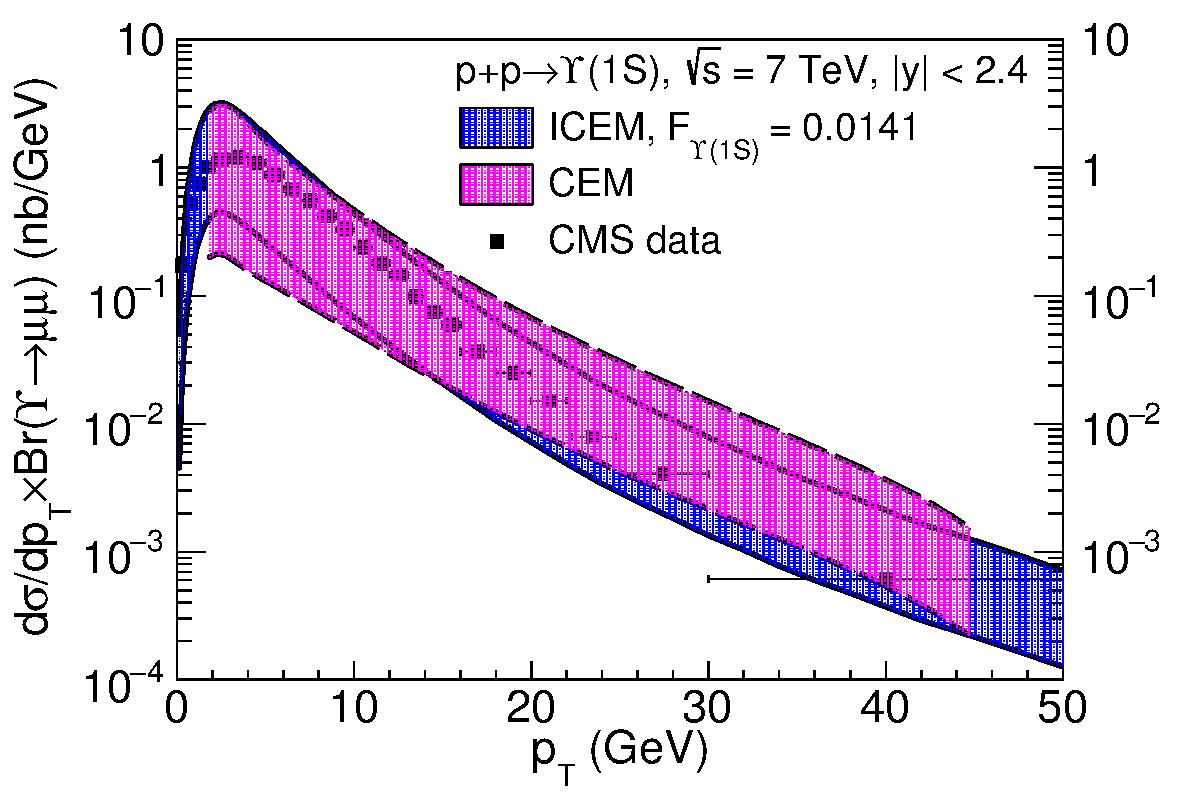
\includegraphics[width=0.60\textwidth]{Figures/RV1S.pdf}
\caption{(Color online) The differential cross section for $\varUpsilon$(1S) production as a function
  of $p_T$ in pp collisions at $\sqrt{s} = 7$~TeV in midrapidity $|y|<2.4$ calcuated using
ICEM~\cite{Cheung:2018upe} with combined mass and renormalization scale
uncertainties (blue).  Also shown the are calculations with CEM using collinear
factorization approach (magenta).
 The calculations are compared with the CMS midrapidity data \cite{Chatrchyan:2013yna}.}
\label{CMS_1S_pt}
\end{figure*}



\begin{figure*}
\centering
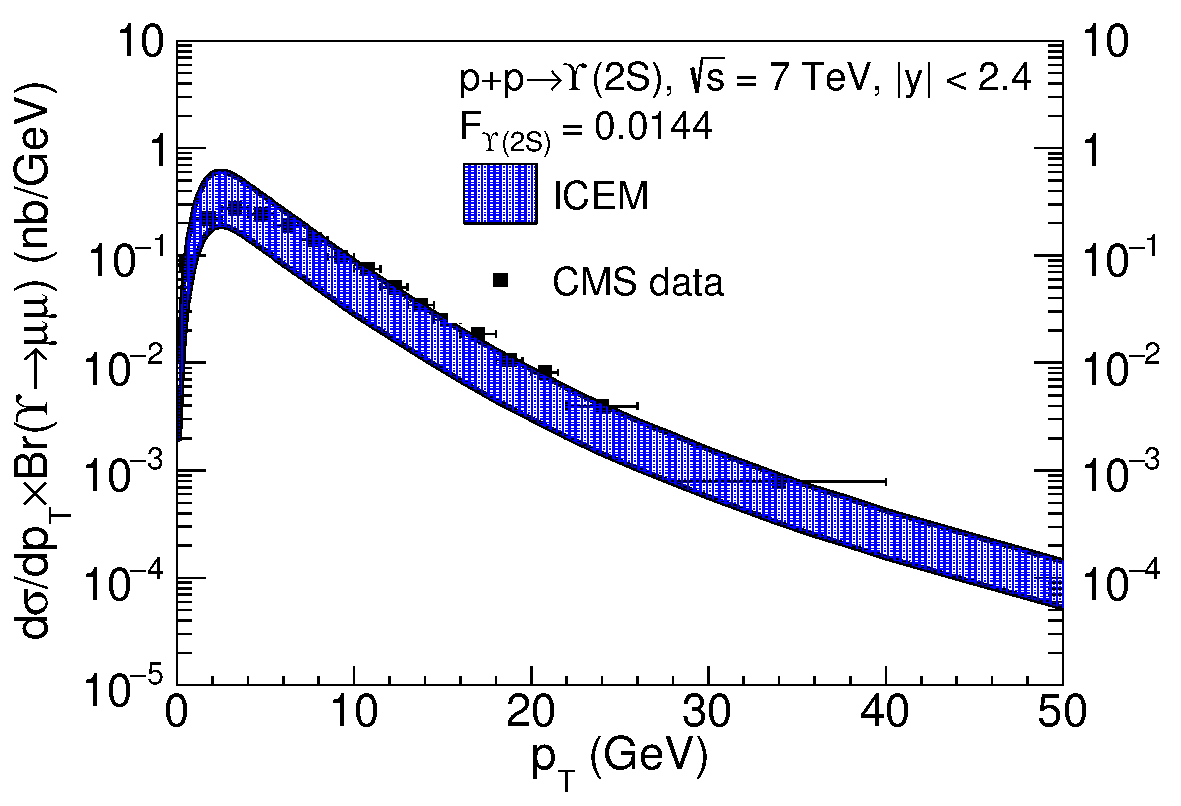
\includegraphics[width=0.48\textwidth]{Figures/RV2S.pdf}
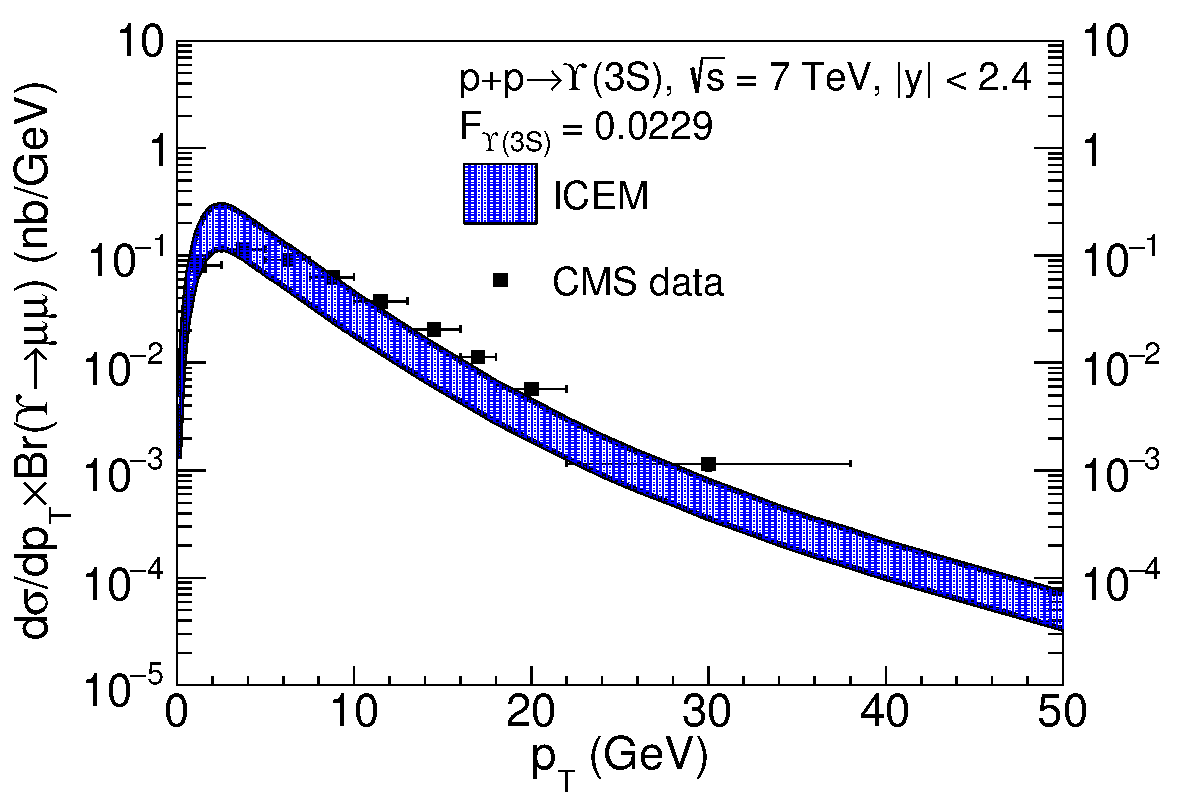
\includegraphics[width=0.48\textwidth]{Figures/RV3S.pdf}
\caption{The differential production cross sections of prompt $\varUpsilon$(2S) (left)
  and prompt $\varUpsilon$(3S) (right) as a function
  of $p_T$ in pp collisions at $\sqrt{s} = 7$~TeV in midrapidity, $|y|<2.4$
  calculated using ICEM~\cite{Cheung:2018upe} with combined mass and renormalization
  scale uncertainties compared with the CMS midrapidity data \cite{Chatrchyan:2013yna}.}
\label{CMS_2S_3S_pt}
\end{figure*}








\subsection{The NRQCD factorization approach}


In the framework of CSM, the $Q\bar{Q}$ pair, eventually evolving into the quarkonium,
is assumed to be in Colour Singlet (CS) state and that has spin and 
angular momentum same as that of quarkonium.
Apart from comprising of the CSM, the NRQCD factorisation approach incorporates 
the Colour Octet (CO) states as well.

In the formalism of the NRQCD factorisation approach, the evolution probability of $Q\bar{Q}$
pair into a state of quarkonium is expressed as matrix elements of NRQCD operators expanded
in terms of heavy quark velocity $v$ (for $v\ll$1)~\cite{Bodwin:1994jh}.
%The NRQCD formalism based on an effective field 
%theory framework, separates the short distance annihilation scale of heavy 
%quarkonium states from long distance ones corresponding to quarkonium structure.
The factorisation formulae are then used to calculate production cross-sections
and decay rates of quarkonia states.
%S-wave states at Next to leading order (NLO) and of P-wave
%states at Leading order (LO).
The full structure of the $Q\bar{Q}$ Fock space
is considered and spanned by $n$=$^{2s+1}L_J^{[a]}$ state where $s$
is the spin, $L$ is the orbital angular momentum, $J$ is the total angular momentum
and $a$ (colour multiplicity) = 1 for CS and 8 for CO states. 
The produced CO states of $Q\bar{Q}$ pair at short distances emerge as 
CS quarkonia by emitting soft gluons non-perturbatively.
%In case of S-wave quarkonia, the CSM is retrieved in the limit of $v\rightarrow$0.
%The short distance cross-sections are obtained theoretically
%using methods of perturbative QCD (pQCD). The long distance matrix elements
%(LDME) that correspond to the probability of 
%$Q\bar{Q}$ pair to emerge as quarkonium are extracted by fitting the measured cross-section
%data.

There have been several works on bottomonia production based on
NRQCD formalism \cite{Domenech:1999qg,Domenech:2000ri,Braaten:2000cm,Gong:2010bk,Sharma:2012dy}.
%In Ref.~\cite{Domenech:1999qg}, a Monte Carlo framework has first
%been employed with CO mechanism for inclusive bottomonia production and few
%NRQCD CO matrix elements for $\Upsilon$(1S) have been extracted at the Tevatron energy. 
%The study has been extended to the whole $\Upsilon$(nS) family in Ref.~\cite{Domenech:2000ri}
%to find CO matrix elements using CDF measurements at Tevatron.
%In Ref.~\cite{Braaten:2000cm} the CO matrix elements are obtained for $\Upsilon$(nS) family
%and the feed downs from $\chi_{b}$(1P) and $\chi_{b}$(2P) to $\Upsilon$(1S) have been 
%considered.
%In Ref.~\cite{Gong:2010bk}, the $\Upsilon$ production has been obtained via
%S-wave CO states calculated at Next to Leading Order (NLO). The LDMEs are obtained
%by fitting the Tevatron data. The ratios of NLO to LO total cross-sections
%have been obtained at Tevatron and LHC energies. Polarisation of inclusive
%$\Upsilon$ has been obtained albeit with large uncertainties.
%In Ref.~\cite{Sharma:2012dy} both CS and CO states along with
%feed down contributions from higher states have been considered to study the
%quarkonia yields for RHIC and LHC energies.
%Using Collins-Soper-Sterman (CSS) formalism, an extension of the NRQCD prediction
%has been carried forward for heavy quarkonium production
%at low $p_T$ by considering soft gluon resummation at all orders in Ref.~\cite{Sun:2012vc}.
Both production and polarisation of $\Upsilon$(nS) at NLO have been discussed in 
Ref.~\cite{Gong:2013qka} within the framework of NRQCD. The CO matrix elements are obtained
by fitting with experimental data. The study is updated in Ref.~\cite{Feng:2015wka} by considering
feed down from $\chi_{bJ}$(mP) states in $\Upsilon$(nS) production. The yields and
polarisations of $\Upsilon$(nS) measured at Tevatron and LHC are well explained by this work.
The NLO study in Ref.~\cite{Han:2014kxa} describes the yields and polarisations of
$\Upsilon$(nS) at LHC which includes feed down contributions from
higher states. In Ref.~\cite{Yu:2017pot}, production cross-section for $\Upsilon$(nS),
$\chi_{bJ}$, $\eta_b$ and $h_b$ have been calculated using NRQCD, as produced in hard
photo production and fragmentation processes at LHC energies. 
It is shown that there is a large difference amoung the LDMEs obtained by different
analysis at NLO.

The LO NRQCD calculations for the differential production
cross-sections of $\Upsilon$ states in p+p collisions have been presented
in~\cite{Kumar:2021sek}.
This work uses a large set of data from Tevatron~\cite{Acosta:2001gv} and
LHC~\cite{LHCb:2012aa,Khachatryan:2015qpa,Aad:2012dlq,Chatrchyan:2013yna,Sirunyan:2017qdw} 
to extract the LDMEs required for the $\Upsilon$ production.
It is to be noted that an LO NRQCD analyis is straightforward and unique and has excellent
predictability power for unknown cross sections.

%and then results are
%presented in Section~\ref{sec:results}.
%A comparison of the obtained LDMEs with the
%previous NRQCD studies both at LO and NLO has been made.
%The summary 
%of our findings are discussed in Section~\ref{sec:summary}. An updated QCD LO study on the
%bottomonia hadroproduction is useful as it provides a reference for comparison
%with NLO calculations. 

The processes that govern the production of heavy mesons like bottomonium,
can be denoted generically by 
$i+j\rightarrow \Upsilon +X$, where $i$ and $j$ are the incident light partons,
$\Upsilon$ is the heavy meson and $X$ is final state light parton.
The double differential cross-section as a function of $p_T$ and rapidity ($y$) of 
the heavy meson can be written as~\cite{Kumar:2016ojy},
\begin{eqnarray}
  E\,\frac{d^3\sigma^{\Upsilon} }{d^3p} &=& \sum_{q,\overline{q},g} \int dx_1 dx_2 f_{i}^p(x_1,\mu_F^2)
  f_{i}^p(x_2,\mu_F^2) \delta(s+u+t-m^2) {\hat{s} \over \pi} \, \frac{d\sigma}{d\hat{t}}
  \label{eq4}
\end{eqnarray}
where, $f_{i}^p$($f_{j}^p$) are distribution functions of the colliding parton $i(j)$ in
the incident protons as a function of $x_1$($x_2$); the fractions of the total momentum
carried by the incident partons and the scale of factorisation $\mu_F$.
Here $\sqrt{s}$ is the total center of mass energy of the pp system and $m_T~(=\mu_F)$ stands for
the transverse mass, $m_T^2=p_T^2 + M^2$ of the quarkonium.
The ${d\sigma}/{d\hat{t}}$ in Eq.~\ref{eq4} is the parton level cross-section and is
defined as~\cite{Bodwin:1994jh},
\begin{equation}
  \frac{d\sigma}{d\hat{t}} = \frac{d\sigma}{d\hat{t}}(ab\rightarrow Q\bar{Q}(^{2s+1}L_J)+X)
  M_L(Q\bar{Q}(^{2s+1}L_J)\rightarrow \Upsilon)
  \label{eq6}
\end{equation}
The first term in RHS is the short distance contribution, that corresponds to the $Q\bar{Q}$
pair production in specific colour and spin configuration and is calculable using 
perturbative QCD (pQCD)~\cite{Braaten:2000cm,Baier:1983va,Humpert:1986cy,Gastmans:1987be,Cho:1995vh,Cho:1995ce}.
The other term in the RHS of Eq.(\ref{eq6}) is the Long Distance Matrix Element (LDME)
and refers to the probability of the $Q\bar{Q}$ state to convert into a quarkonium state.
They are determined by comparing the calculations with the measurements.




%\begin{figure}
%  \centering
%  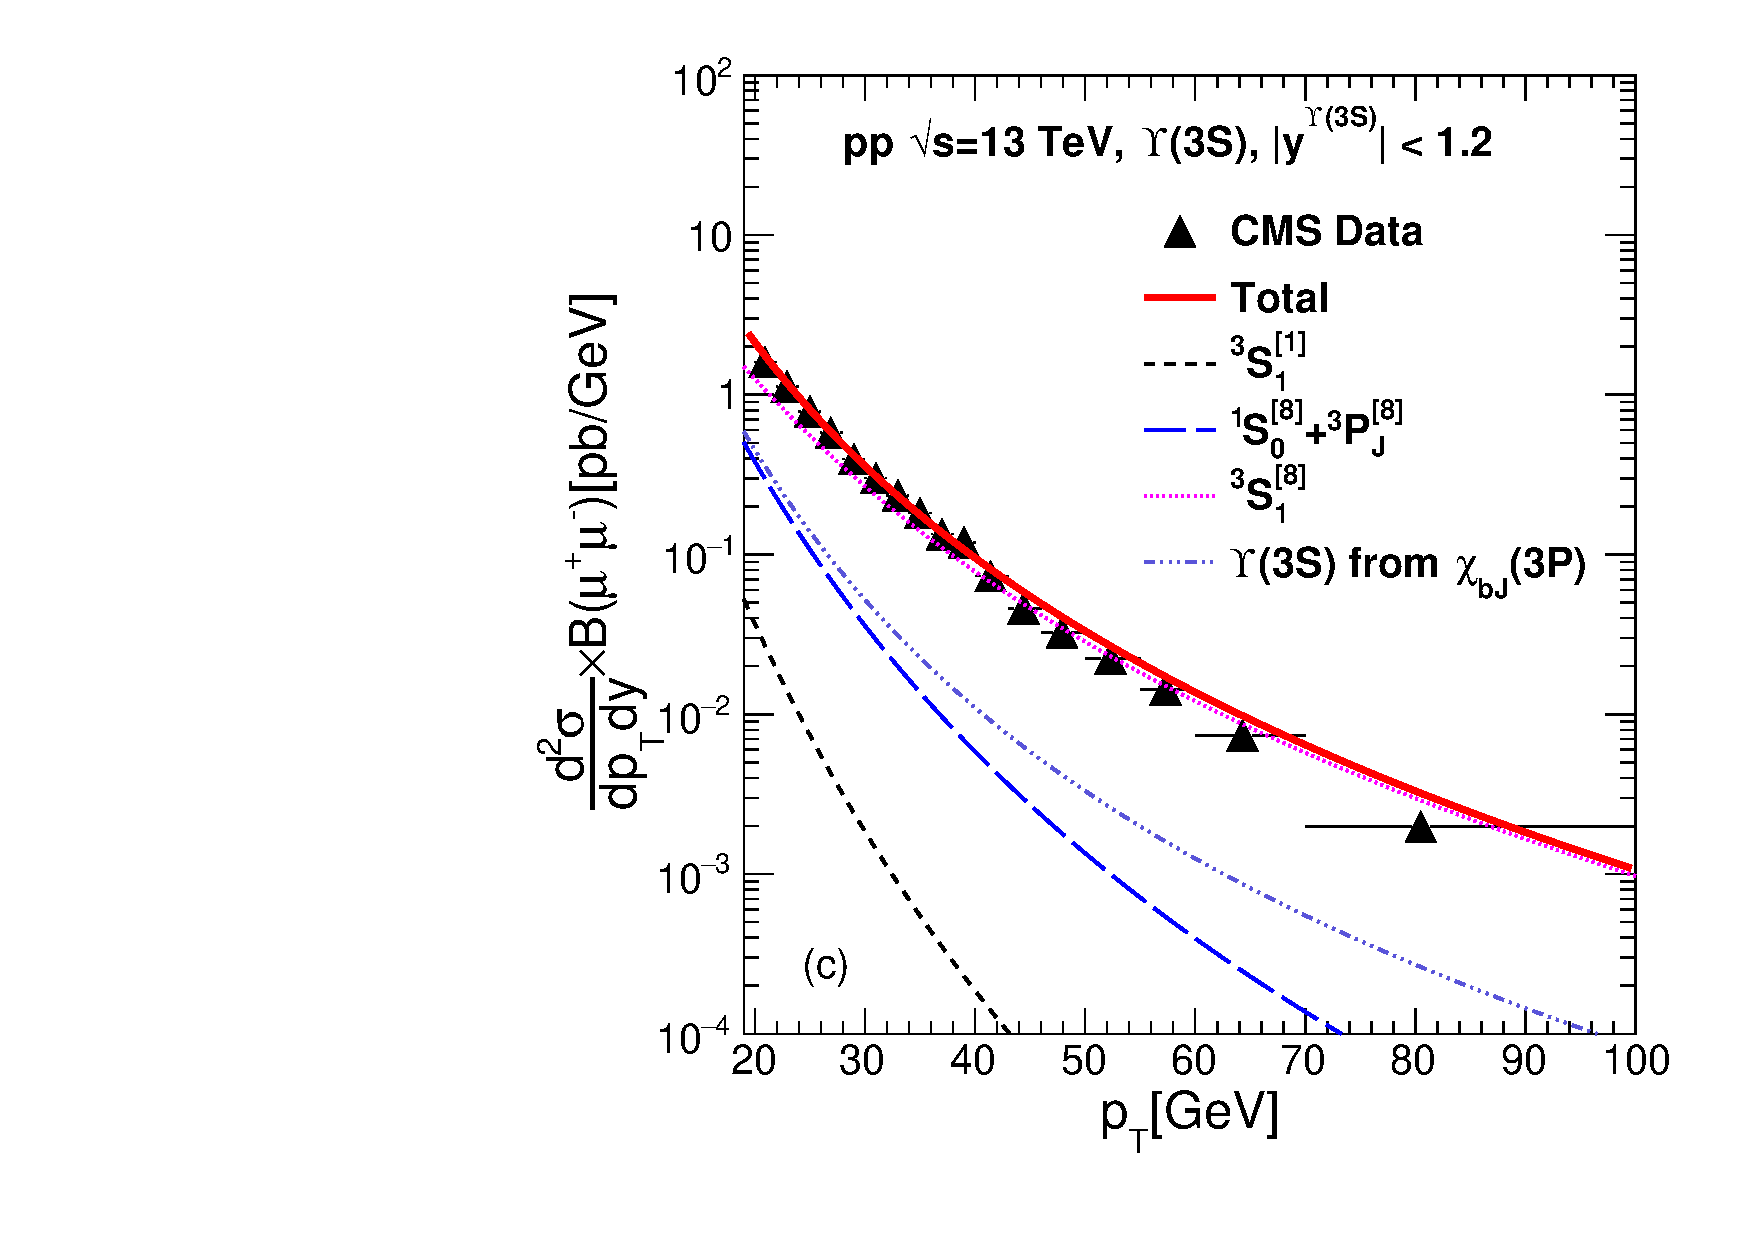
\includegraphics[width=0.49\textwidth]{Figures/NRQCD_Beauty/Fig3c_Y3S_CMS_13TeV_Rap12.pdf}
%  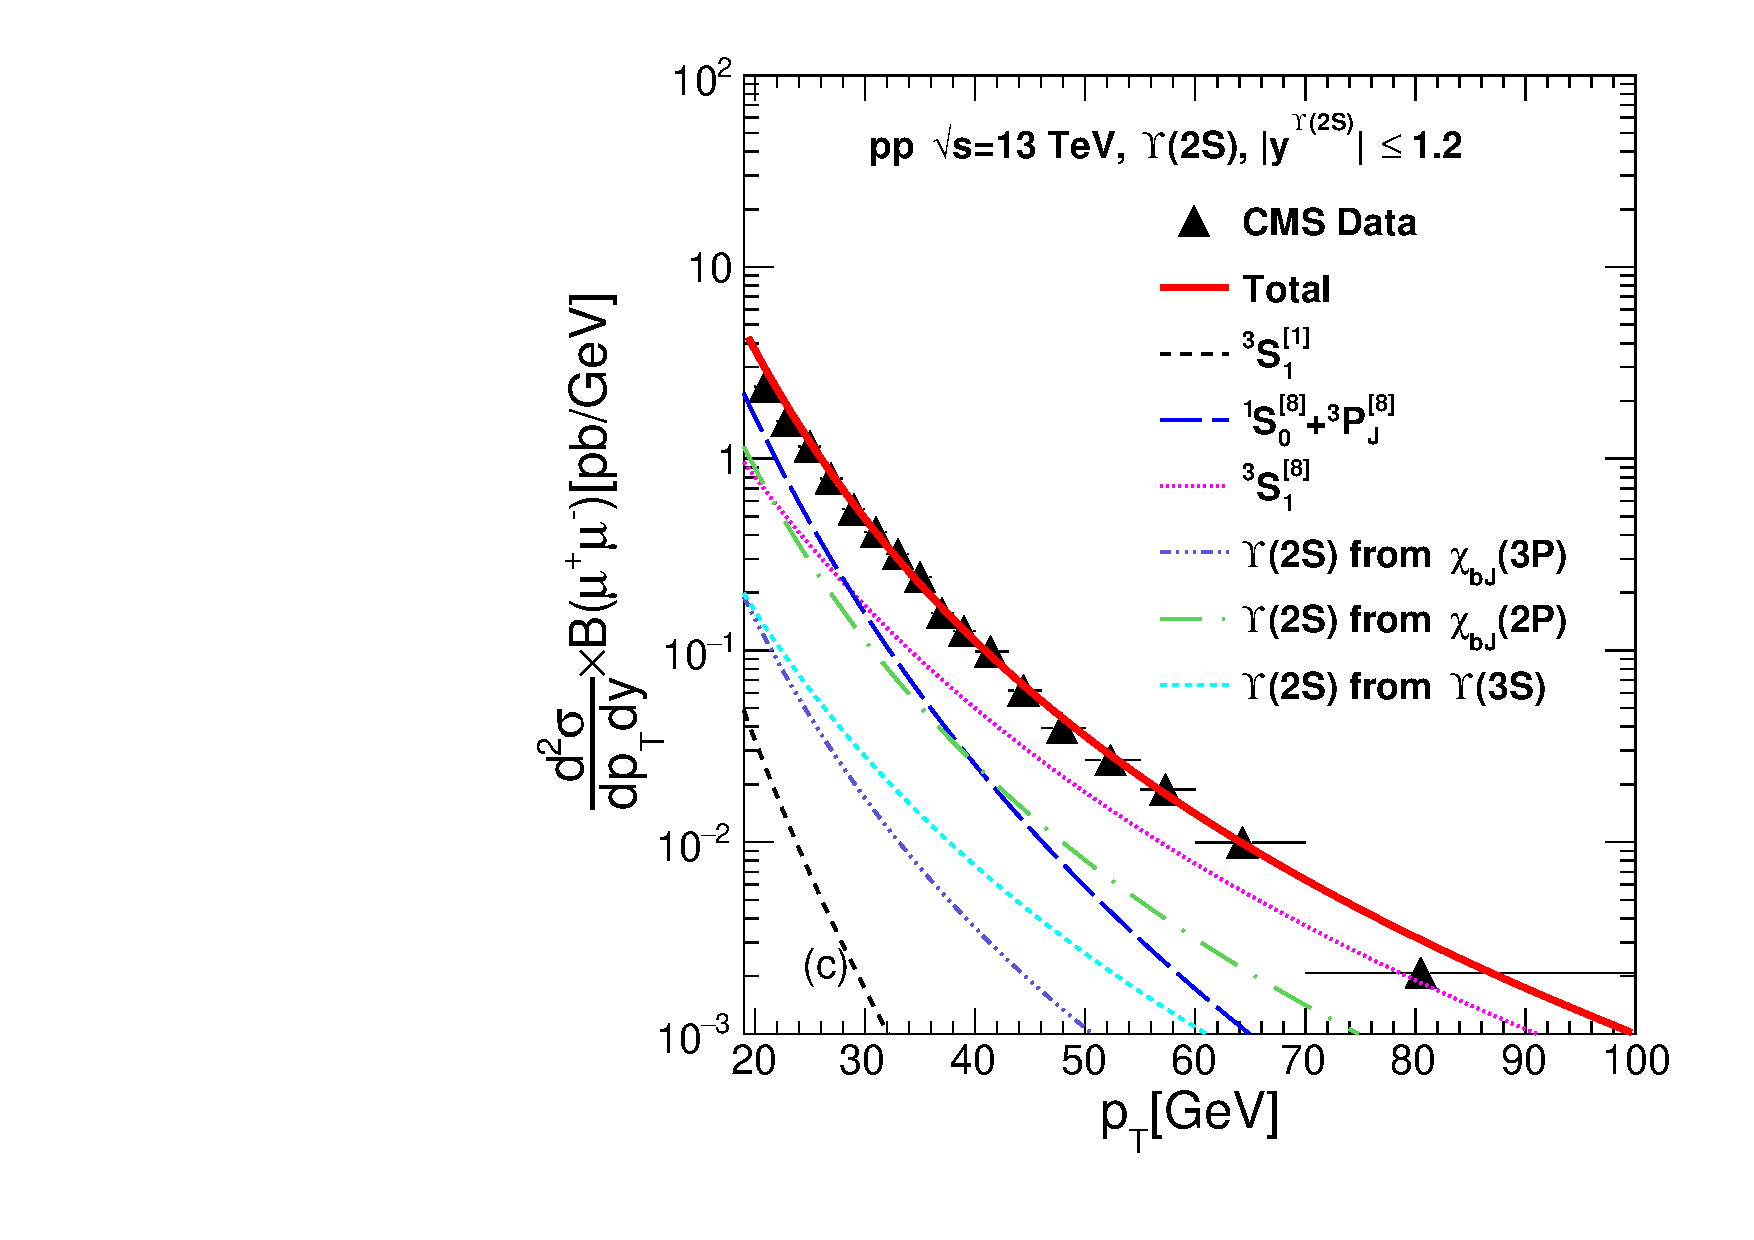
\includegraphics[width=0.49\textwidth]{Figures/NRQCD_Beauty/Fig6c_CMS_D2NDPtDy_Y2S_13TeV_Y0012_Pt.pdf}
%  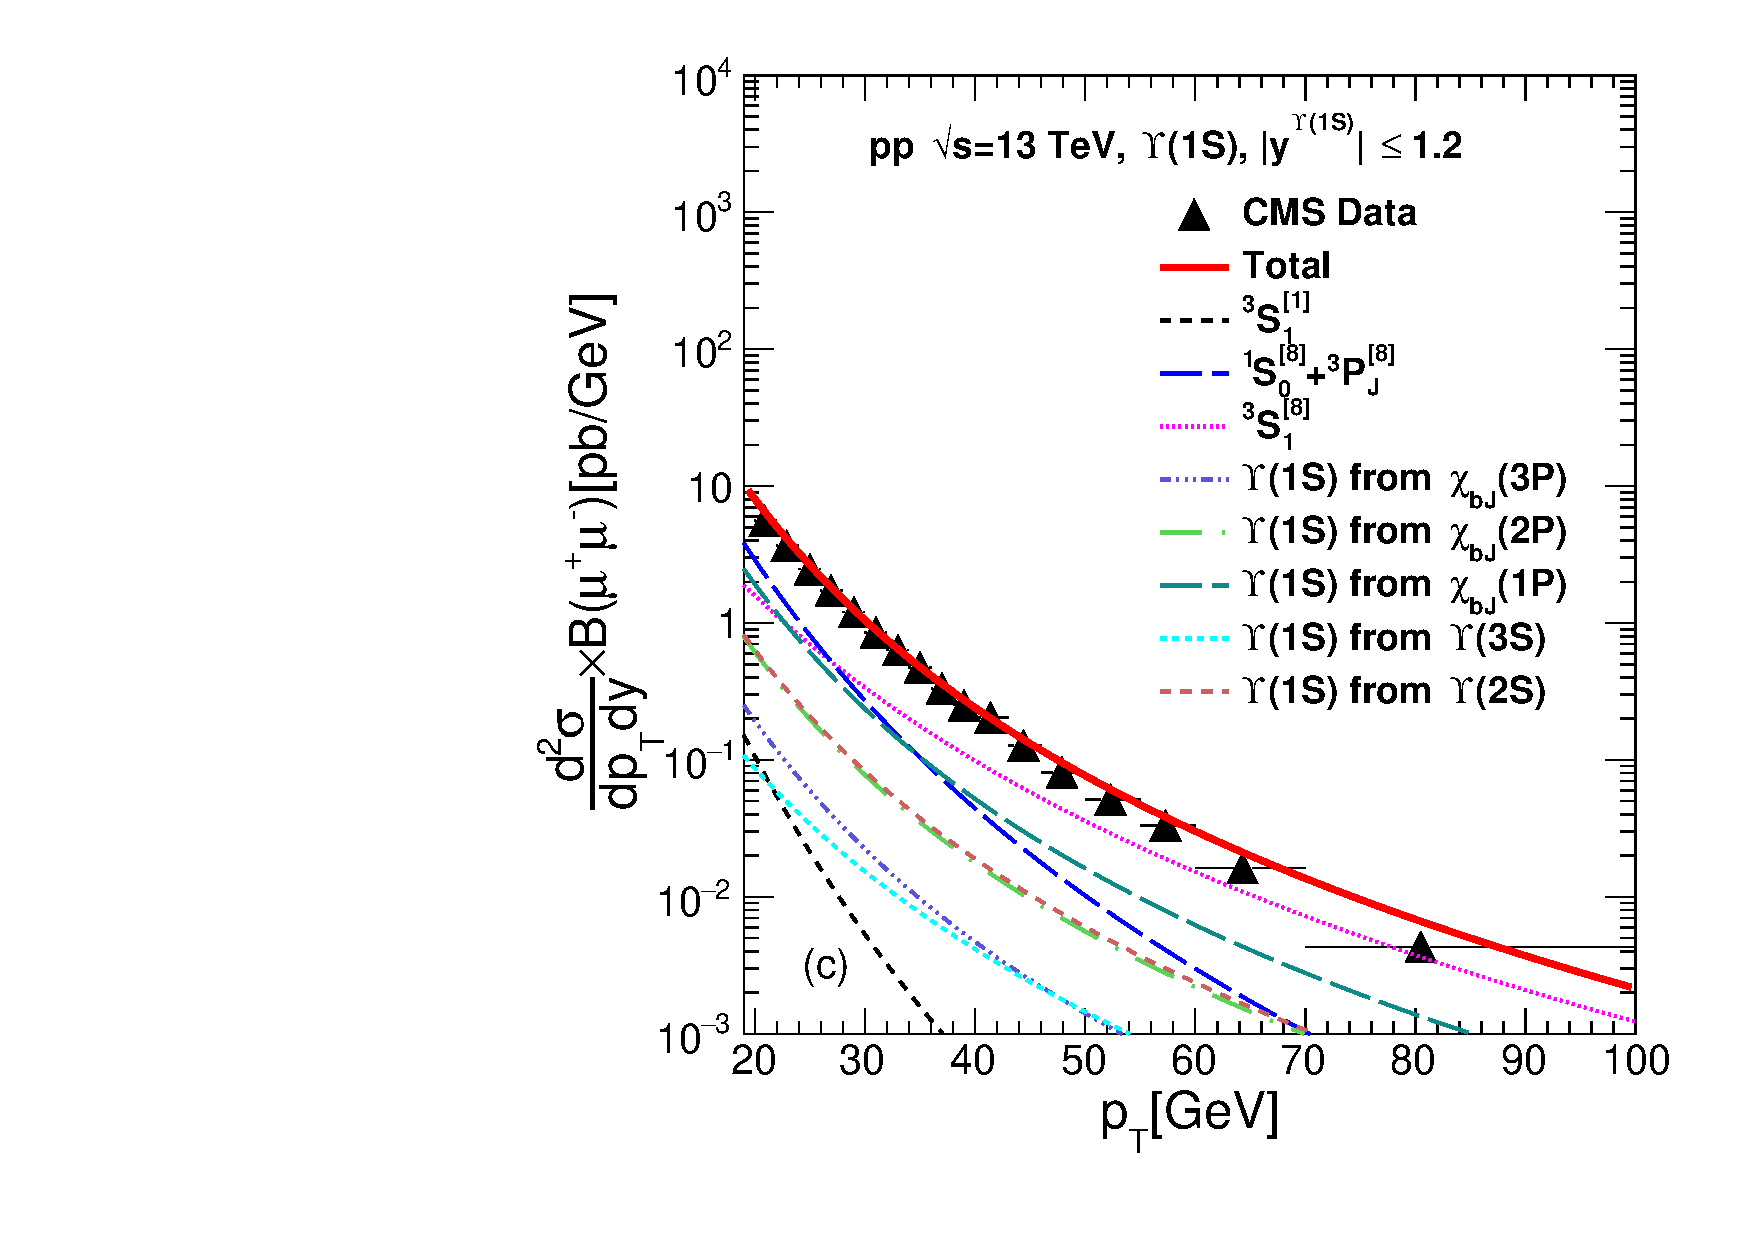
\includegraphics[width=0.49\textwidth]{Figures/NRQCD_Beauty/Fig8c_CMS_D2NDPtDy_Y1S_13TeV_Y0012_Pt.pdf}
%  \caption{\small{The NRQCD calculations of production cross-section of $\Upsilon$(nS) in p+p collisions at 
%      $\sqrt{s}$ = 13 TeV in central rapidities, as a function of transverse momentum compared with the measured data 
%      at CMS~\cite{Sirunyan:2017qdw} experiment.}}
%  %   The LDMEs are obtained by a combined fit of the CMS and ATLAS data.}
%  \label{Fig:SigmaYnSCMS13TeV}
%\end{figure}


%\begin{figure}
%  \centering
%  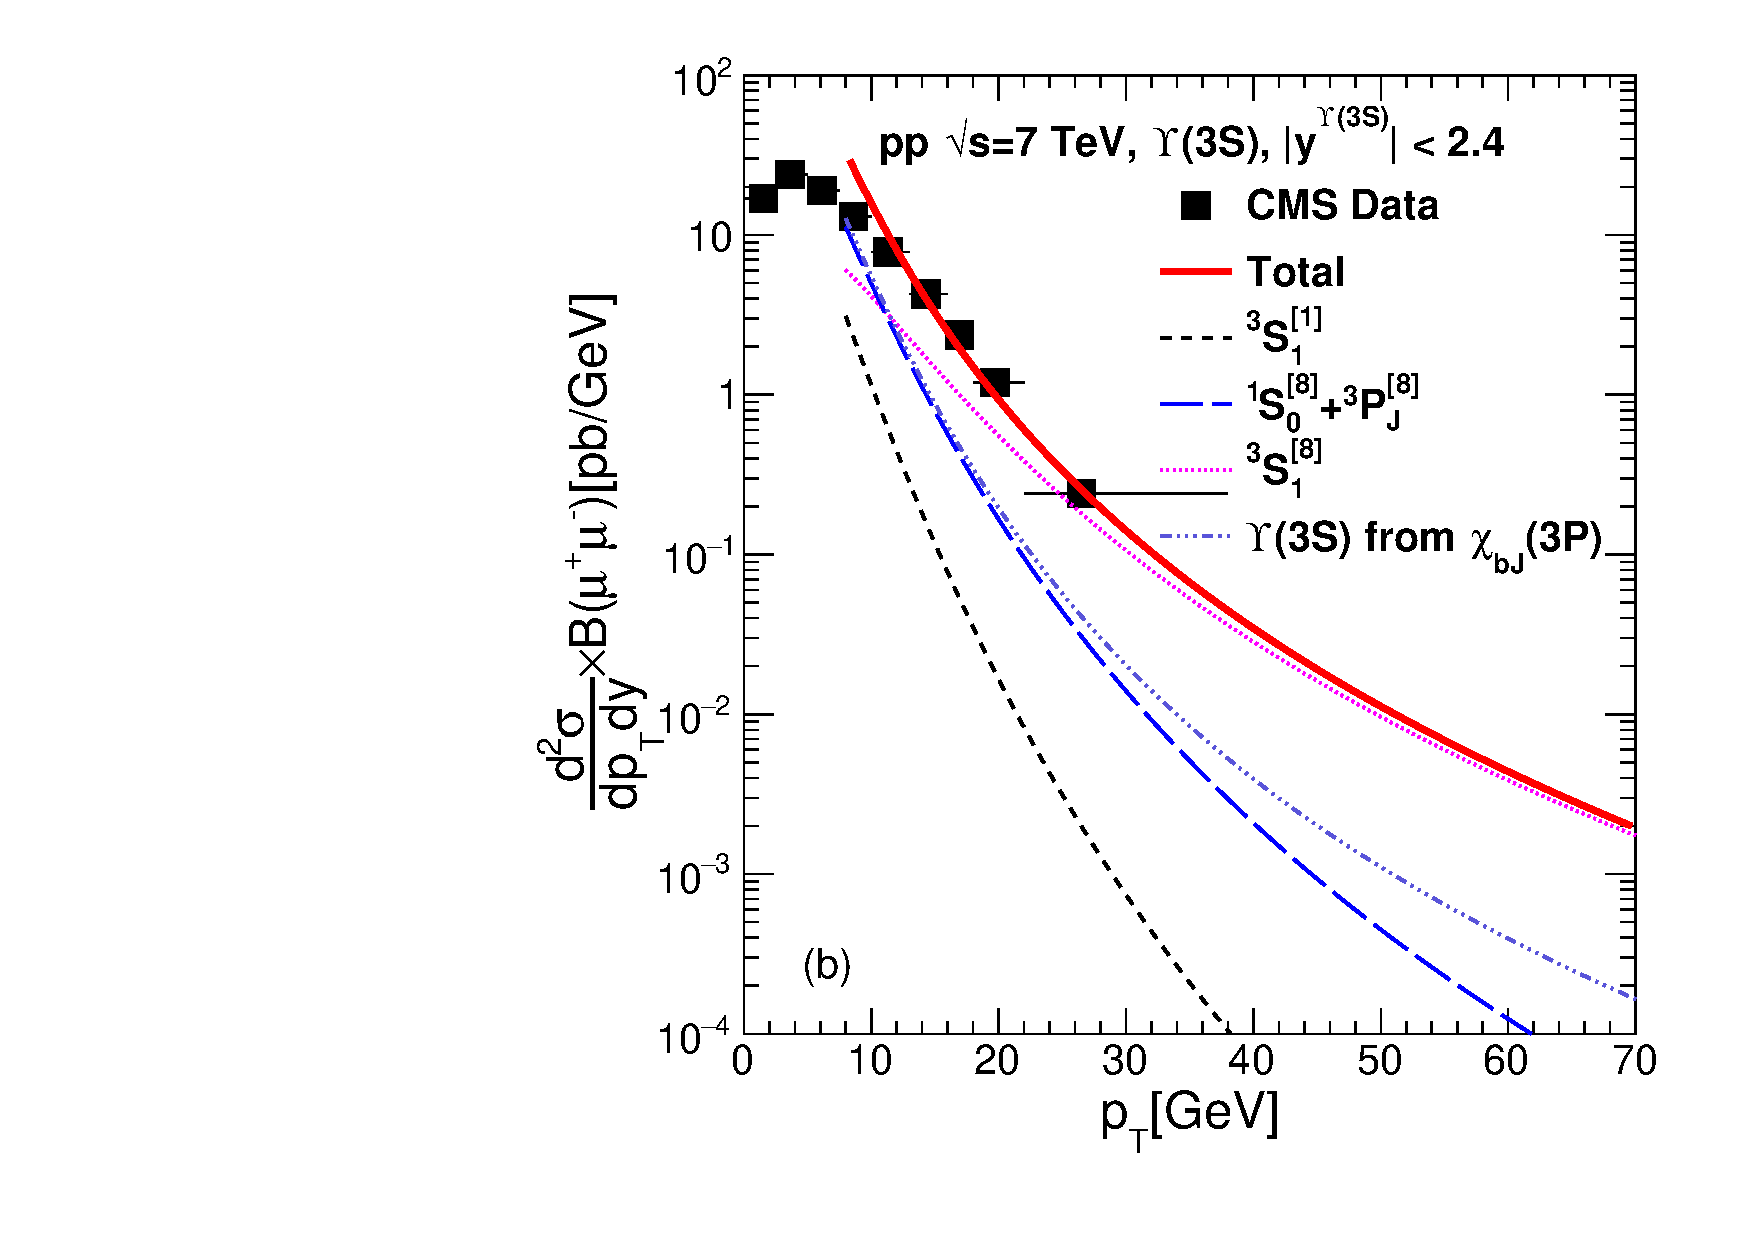
\includegraphics[width=0.49\textwidth]{Figures/NRQCD_Beauty/Fig2b_Y3S_CMS_Rapl24.pdf}
%  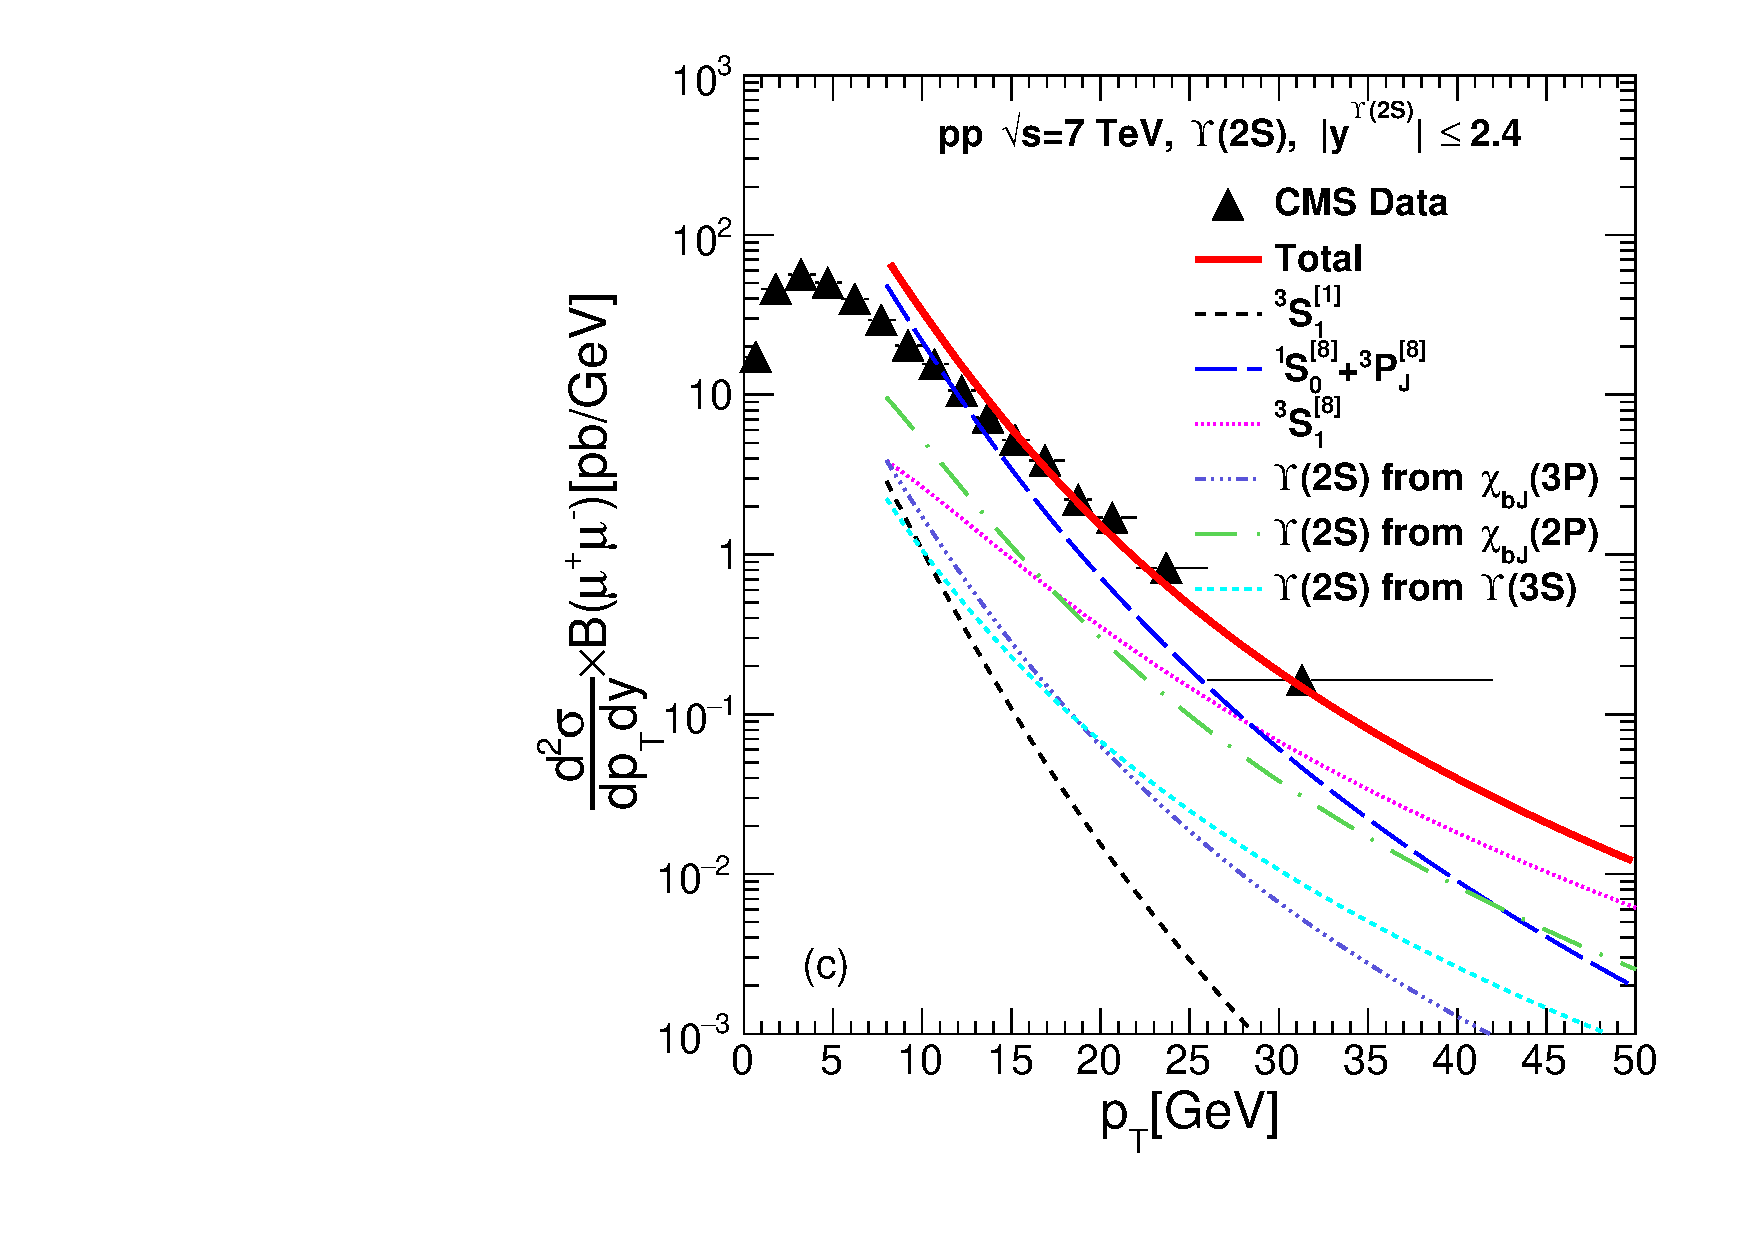
\includegraphics[width=0.49\textwidth]{Figures/NRQCD_Beauty/Fig5c_CMS_D2NDPtDy_Y2S_Y0024_Pt.pdf}
%  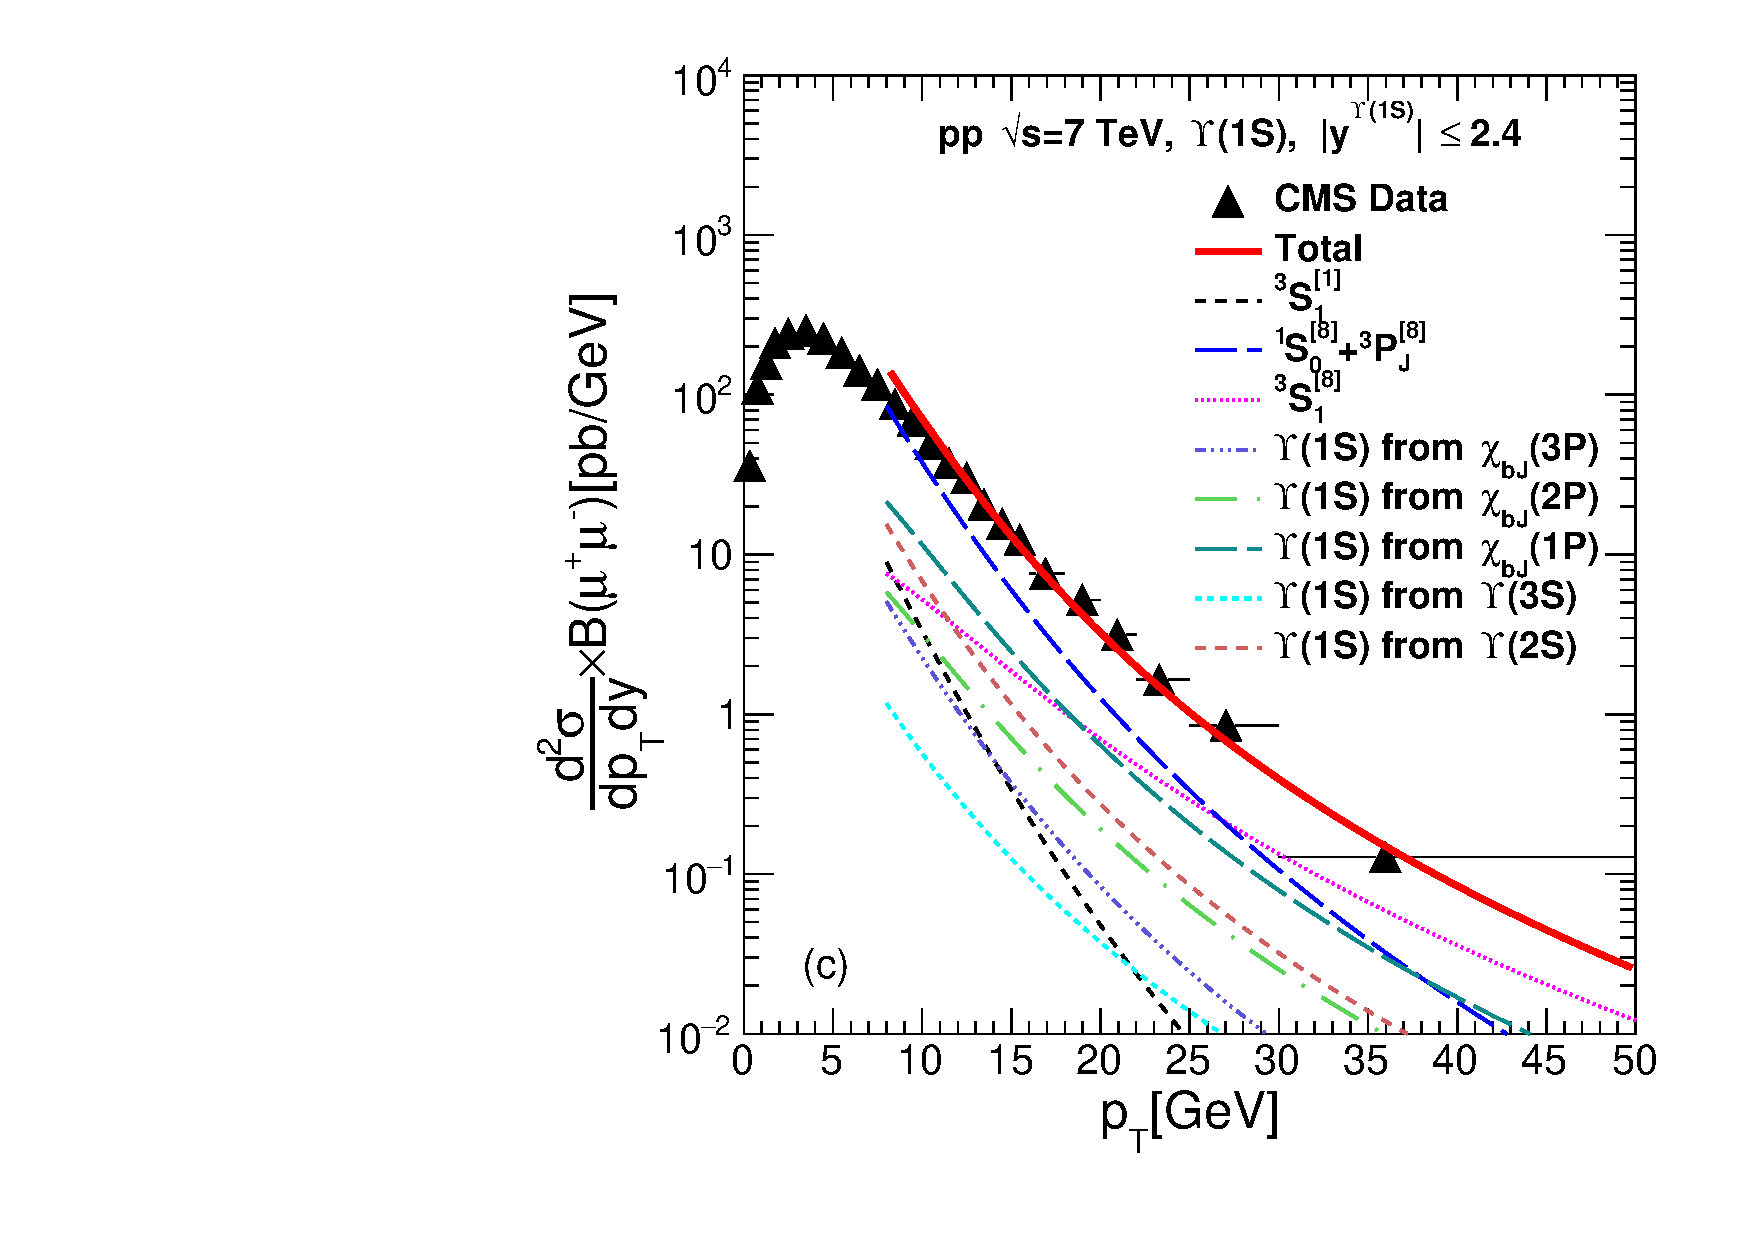
\includegraphics[width=0.49\textwidth]{Figures/NRQCD_Beauty/Fig7c_CMS_D2NDPtDy_Y1S_Y0024_Pt.pdf}
%  \caption{\small{The NRQCD calculations of production cross-section of $\Upsilon$(nS) in p+p collisions at 
%      $\sqrt{s}$ = 7 TeV in central rapidities, as a function of transverse momentum compared with the measured data 
%      at CMS~\cite{Chatrchyan:2013yna} experiment.}}
%  %   The LDMEs are obtained by a combined fit of the CMS and ATLAS data.}
%  \label{Fig:SigmaYnSCMS7TeV}
%\end{figure}

%\begin{figure}
%  \centering
%  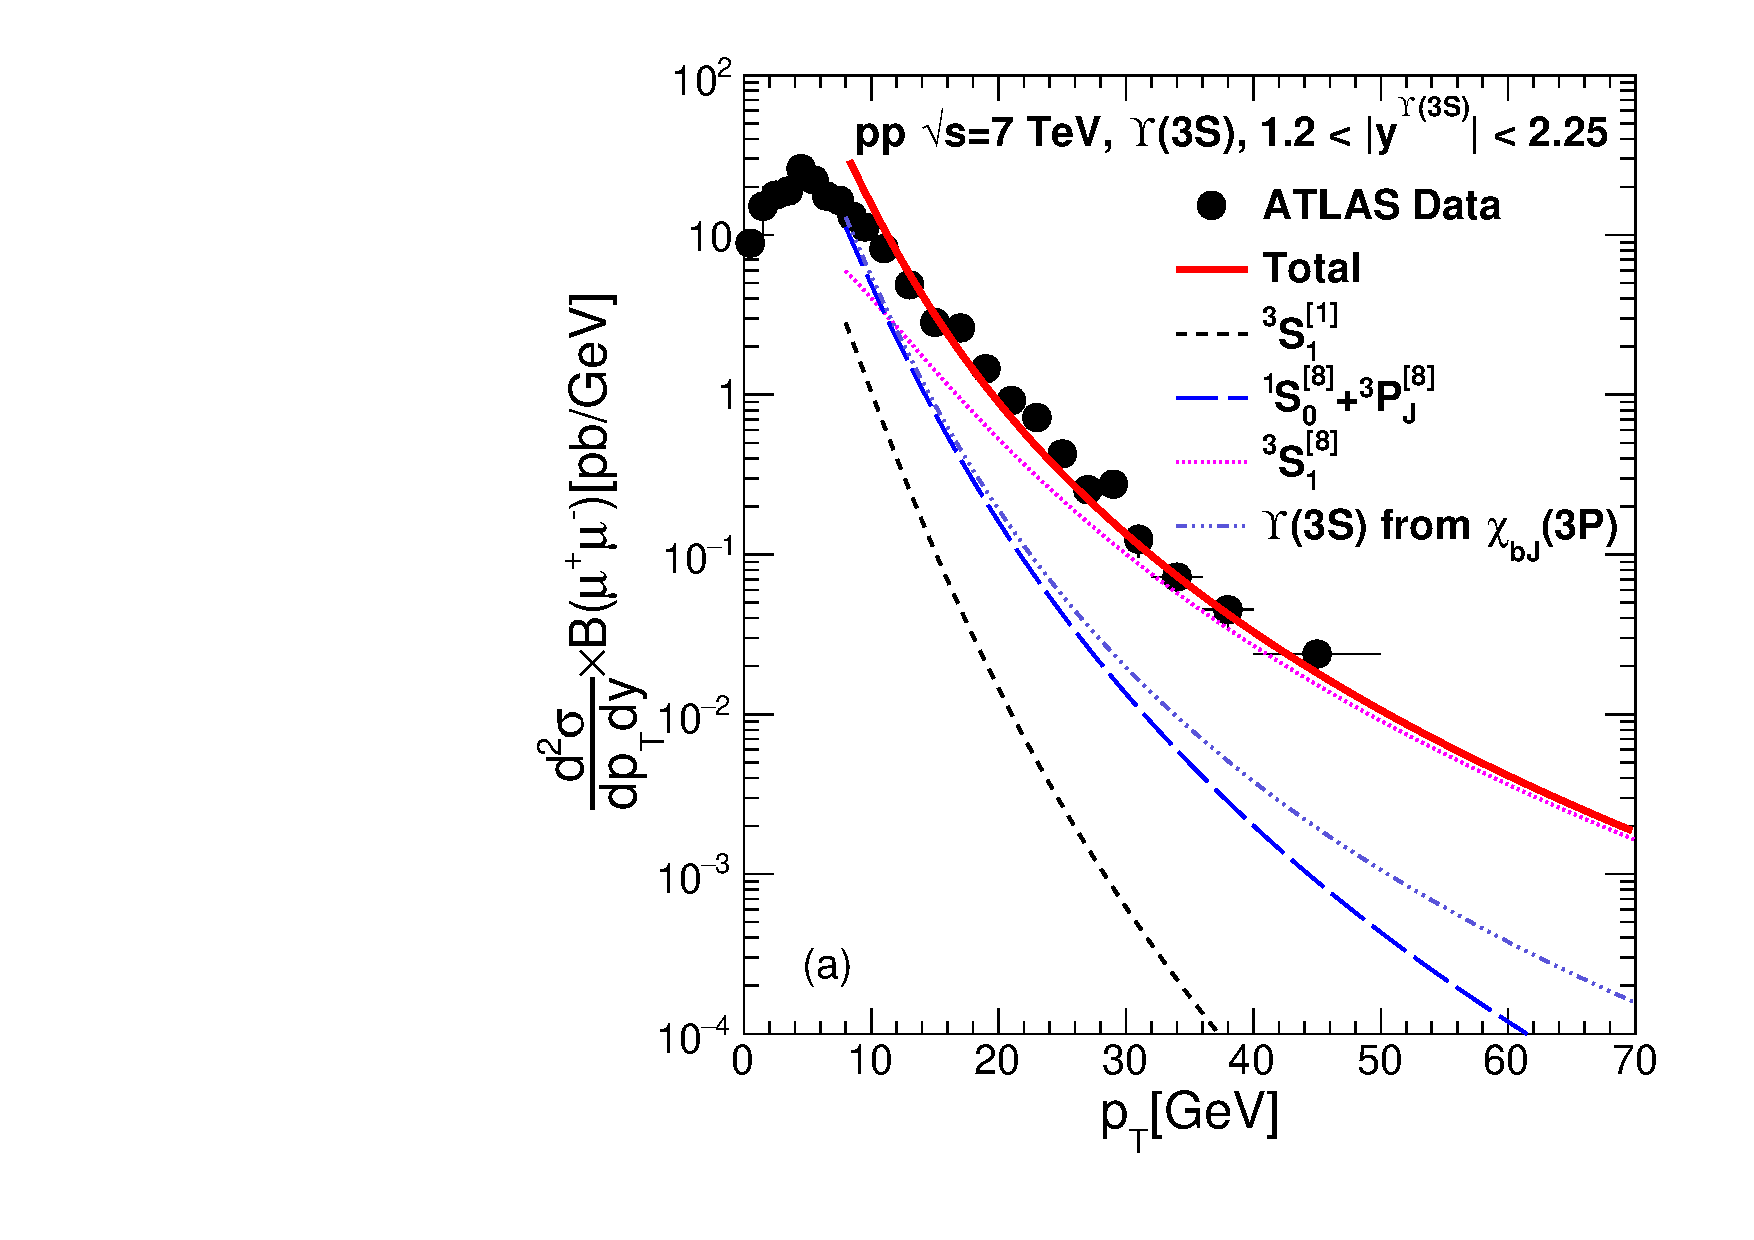
\includegraphics[width=0.49\textwidth]{Figures/NRQCD_Beauty/Fig2a_Y3S_ATLAS_Rap12225.pdf}
%  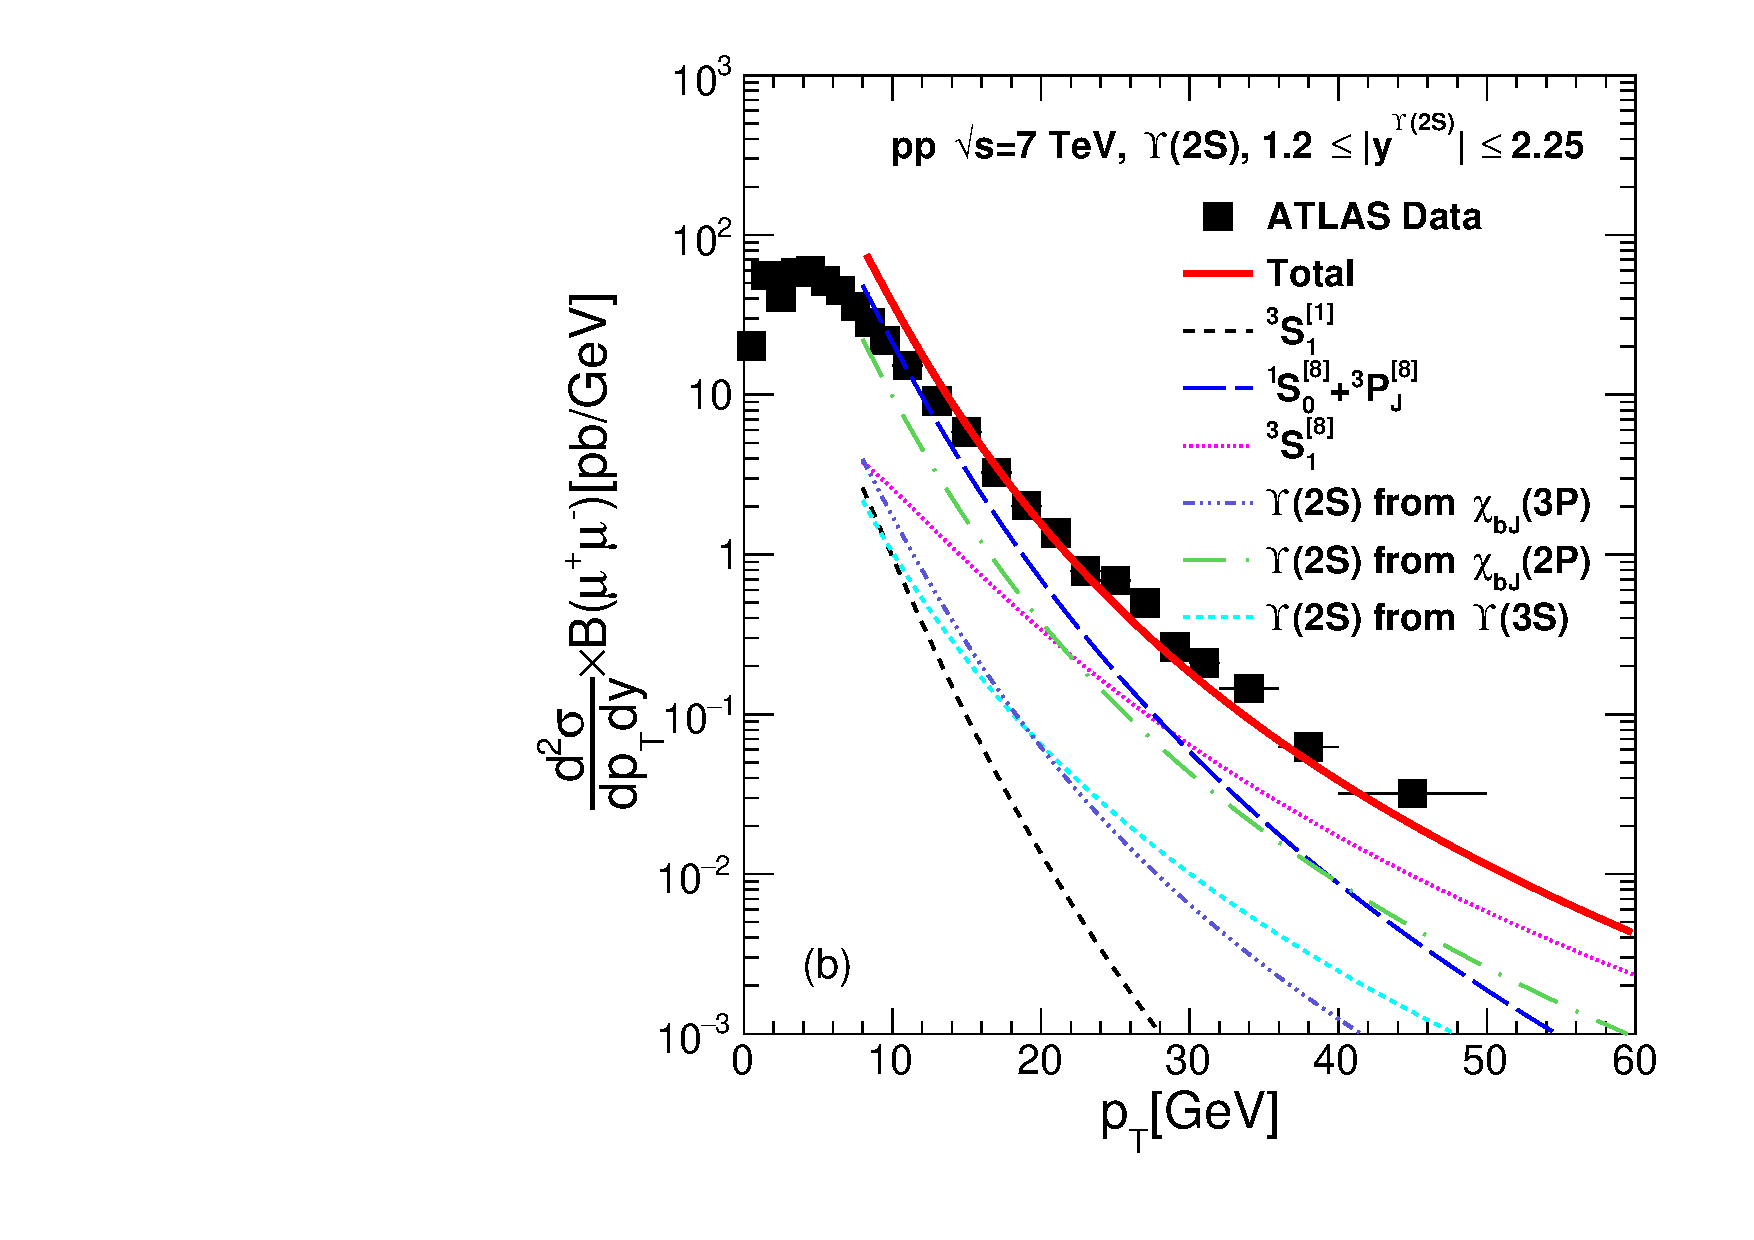
\includegraphics[width=0.49\textwidth]{Figures/NRQCD_Beauty/Fig5b_ATLAS_D2NDPtDy_Y2S_Y12225_Pt.pdf}
%  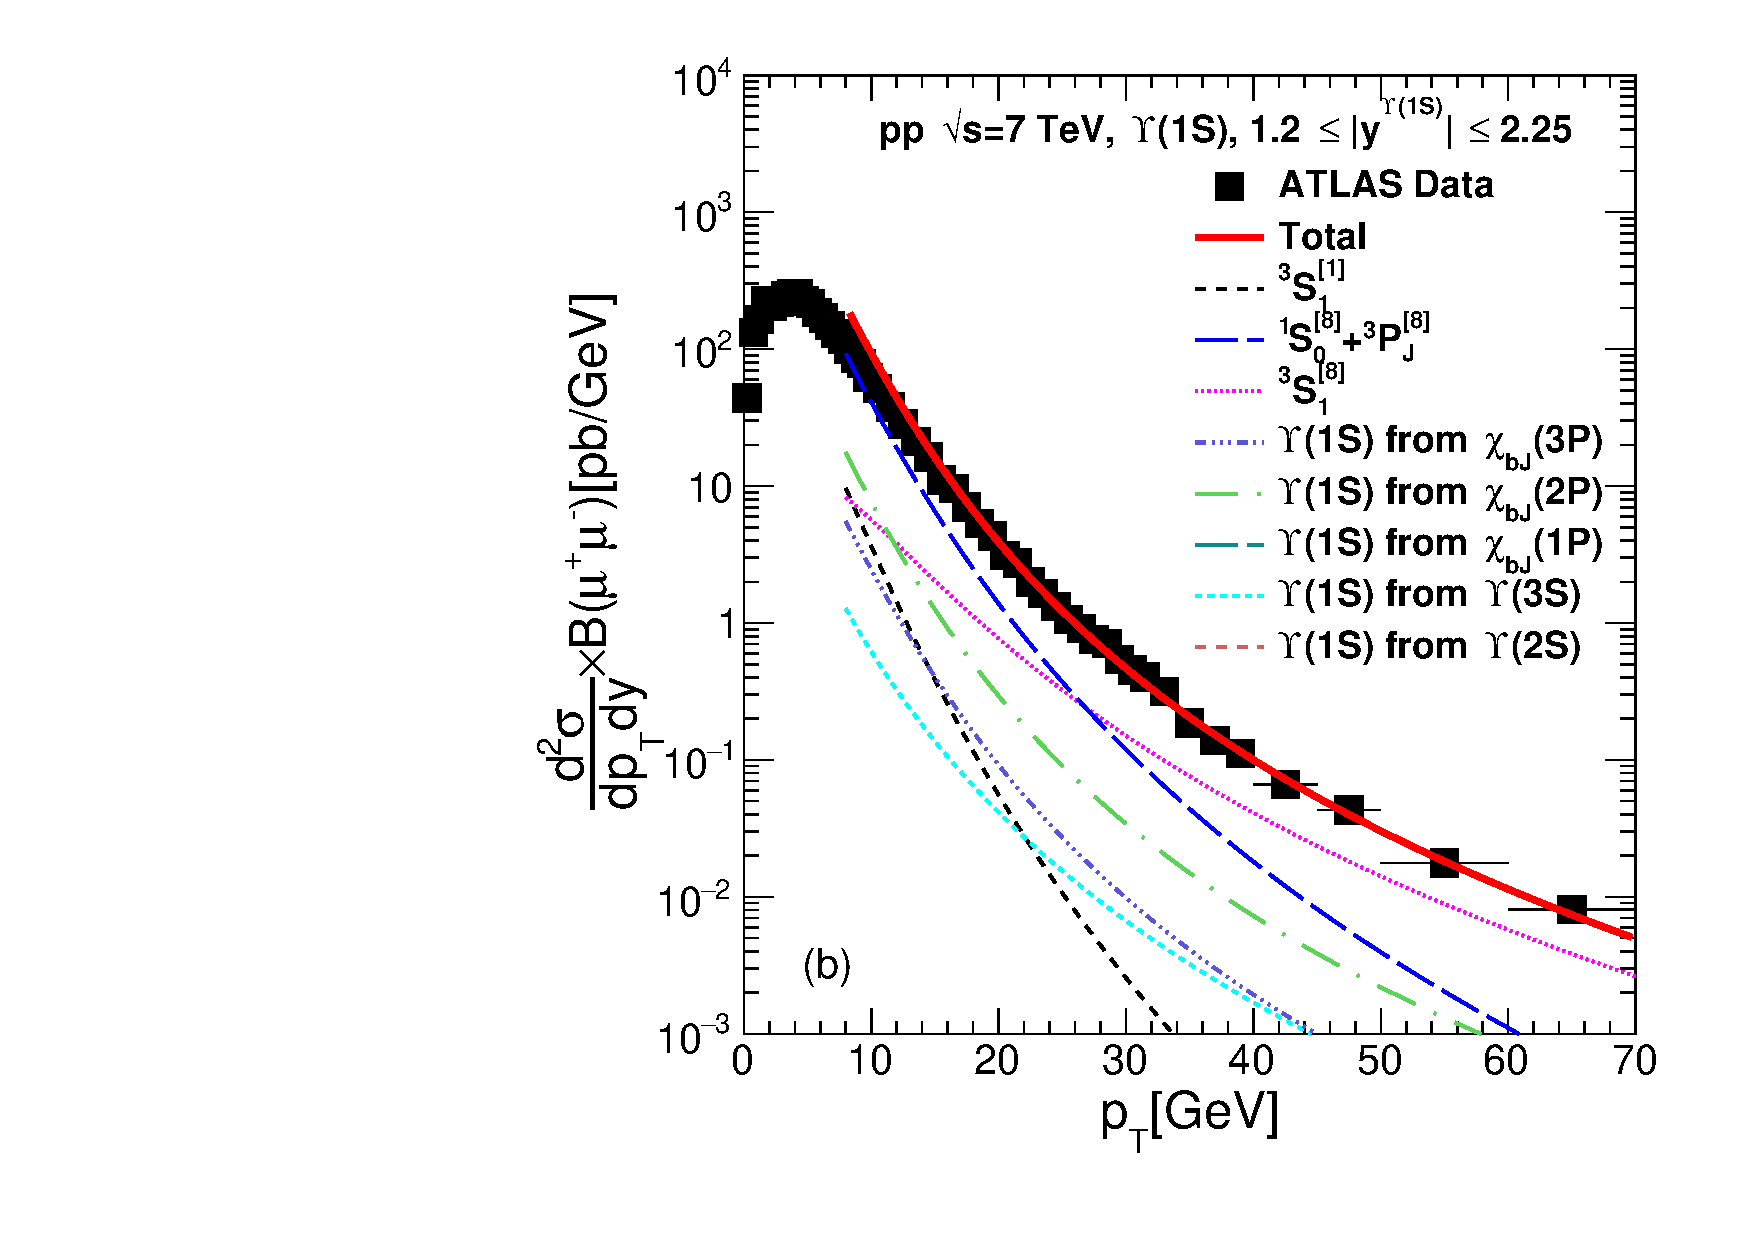
\includegraphics[width=0.49\textwidth]{Figures/NRQCD_Beauty/Fig7b_ATLAS_D2NDPtDy_Y1S_Y12225_Pt.pdf}
%  \caption{\small{The NRQCD calculations of production cross-section of $\Upsilon$(nS) in p+p collisions at 
%      $\sqrt{s}$ = 7 TeV in central rapidities, as a function of transverse momentum compared with the measured data 
%      at ATLAS~\cite{Aad:2012dlq} experiment.}}
%  %   The LDMEs are obtained by a combined fit of the CMS and ATLAS data.}
%  \label{Fig:SigmaYnSATLAS7TeV}
%\end{figure}


\begin{figure}
  \centering
  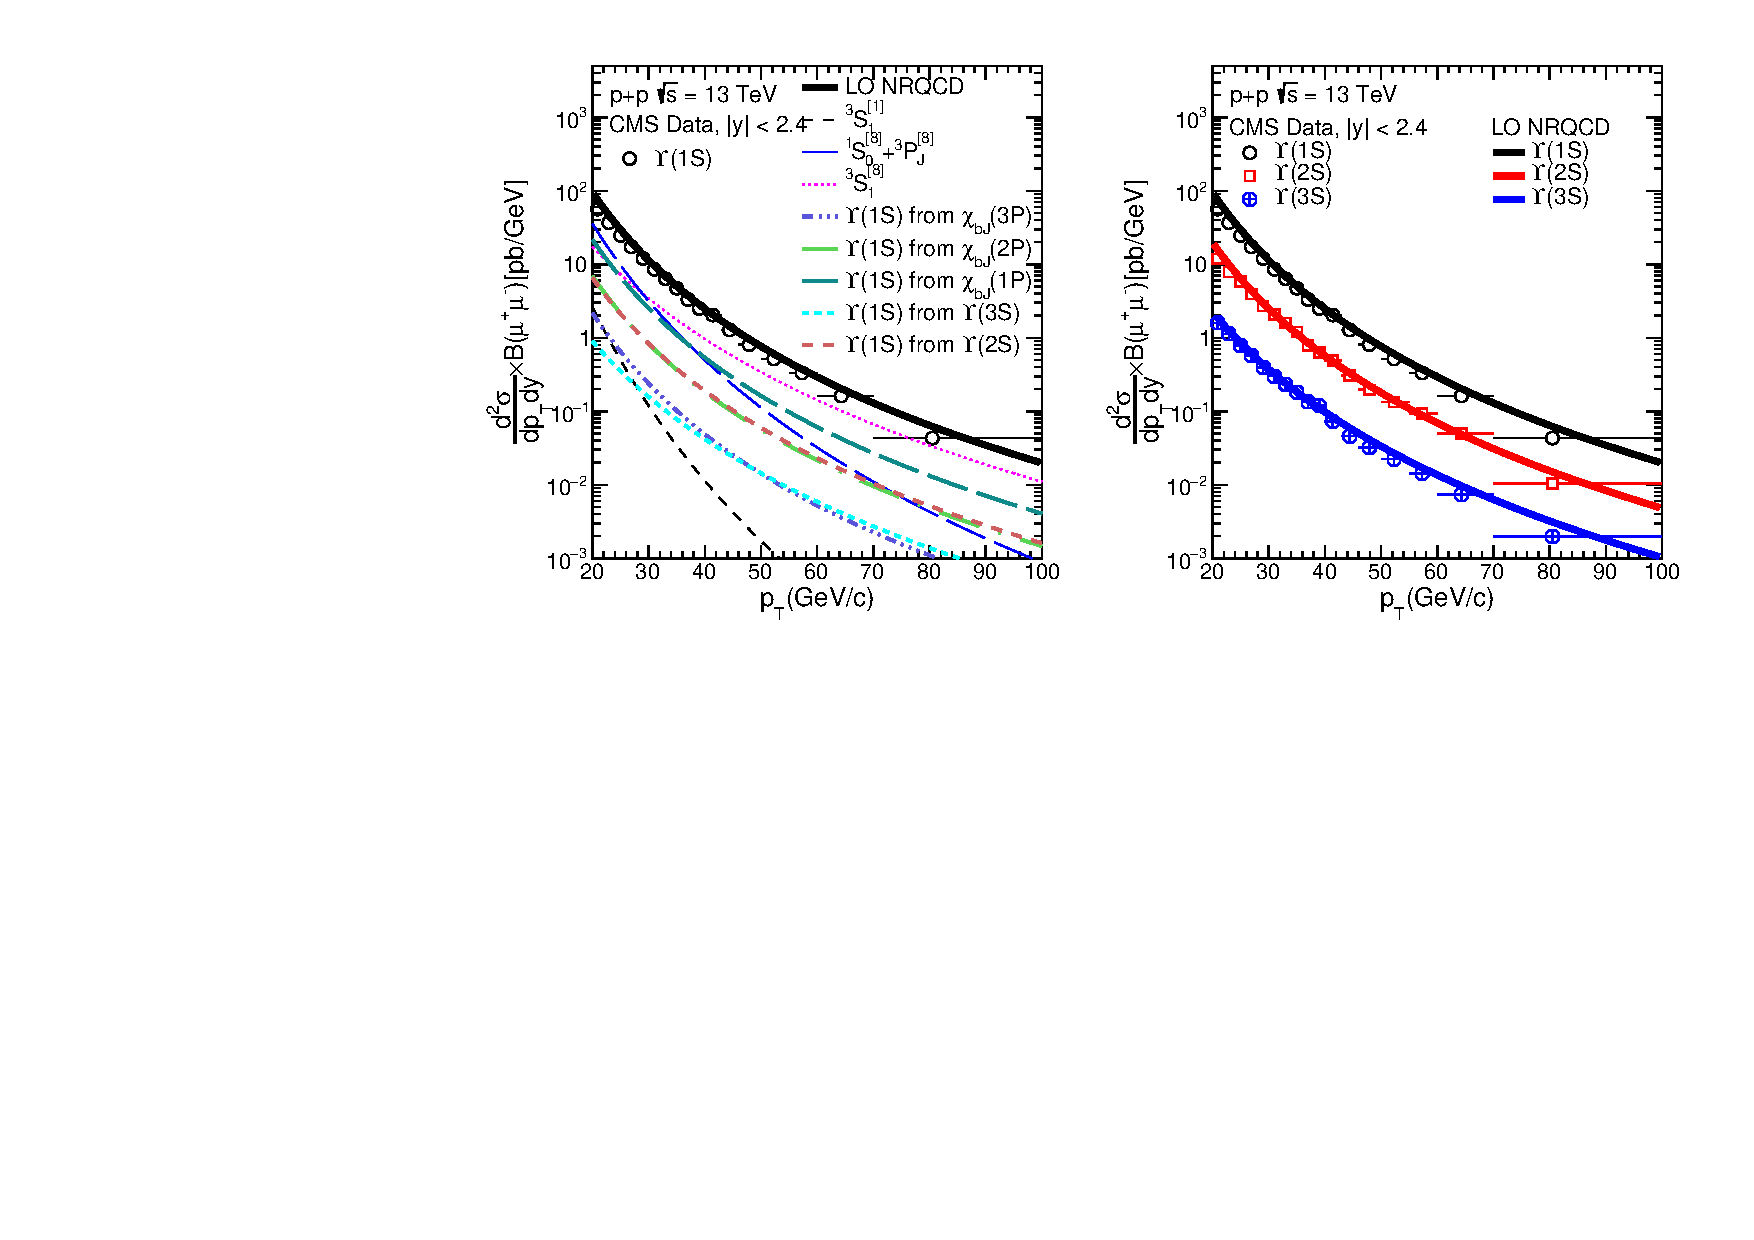
\includegraphics[width=0.99\textwidth]{Figures/NRQCD_Beauty/Fig_CMS_YnS_Rap12_13TeV_Pt.pdf}
  \caption{\small{The NRQCD calculations~\cite{Kumar:2021sek} of production cross-section of $\Upsilon$(nS)
      in p+p collisions at $\sqrt{s}$ = 13 TeV in central rapidities, as a function of
      transverse momentum compared with the measured data at CMS~\cite{Sirunyan:2017qdw}
      experiment. The left figure shows relative contributions in $\Upsilon$(1S) from
      singlet and octet states as well as from feeddown. The right figure shows the sum
      of all contributions for all the 3 states where the results for $\Upsilon$(1S) and
      $\Upsilon$(2S) are shifted vertically by a constant factor for better visibility. } }
  %   The LDMEs are obtained by a combined fit of the CMS and ATLAS data.}
  \label{Fig:SigmaYnSCMS13TeV}
\end{figure}



\begin{figure}
  \centering
  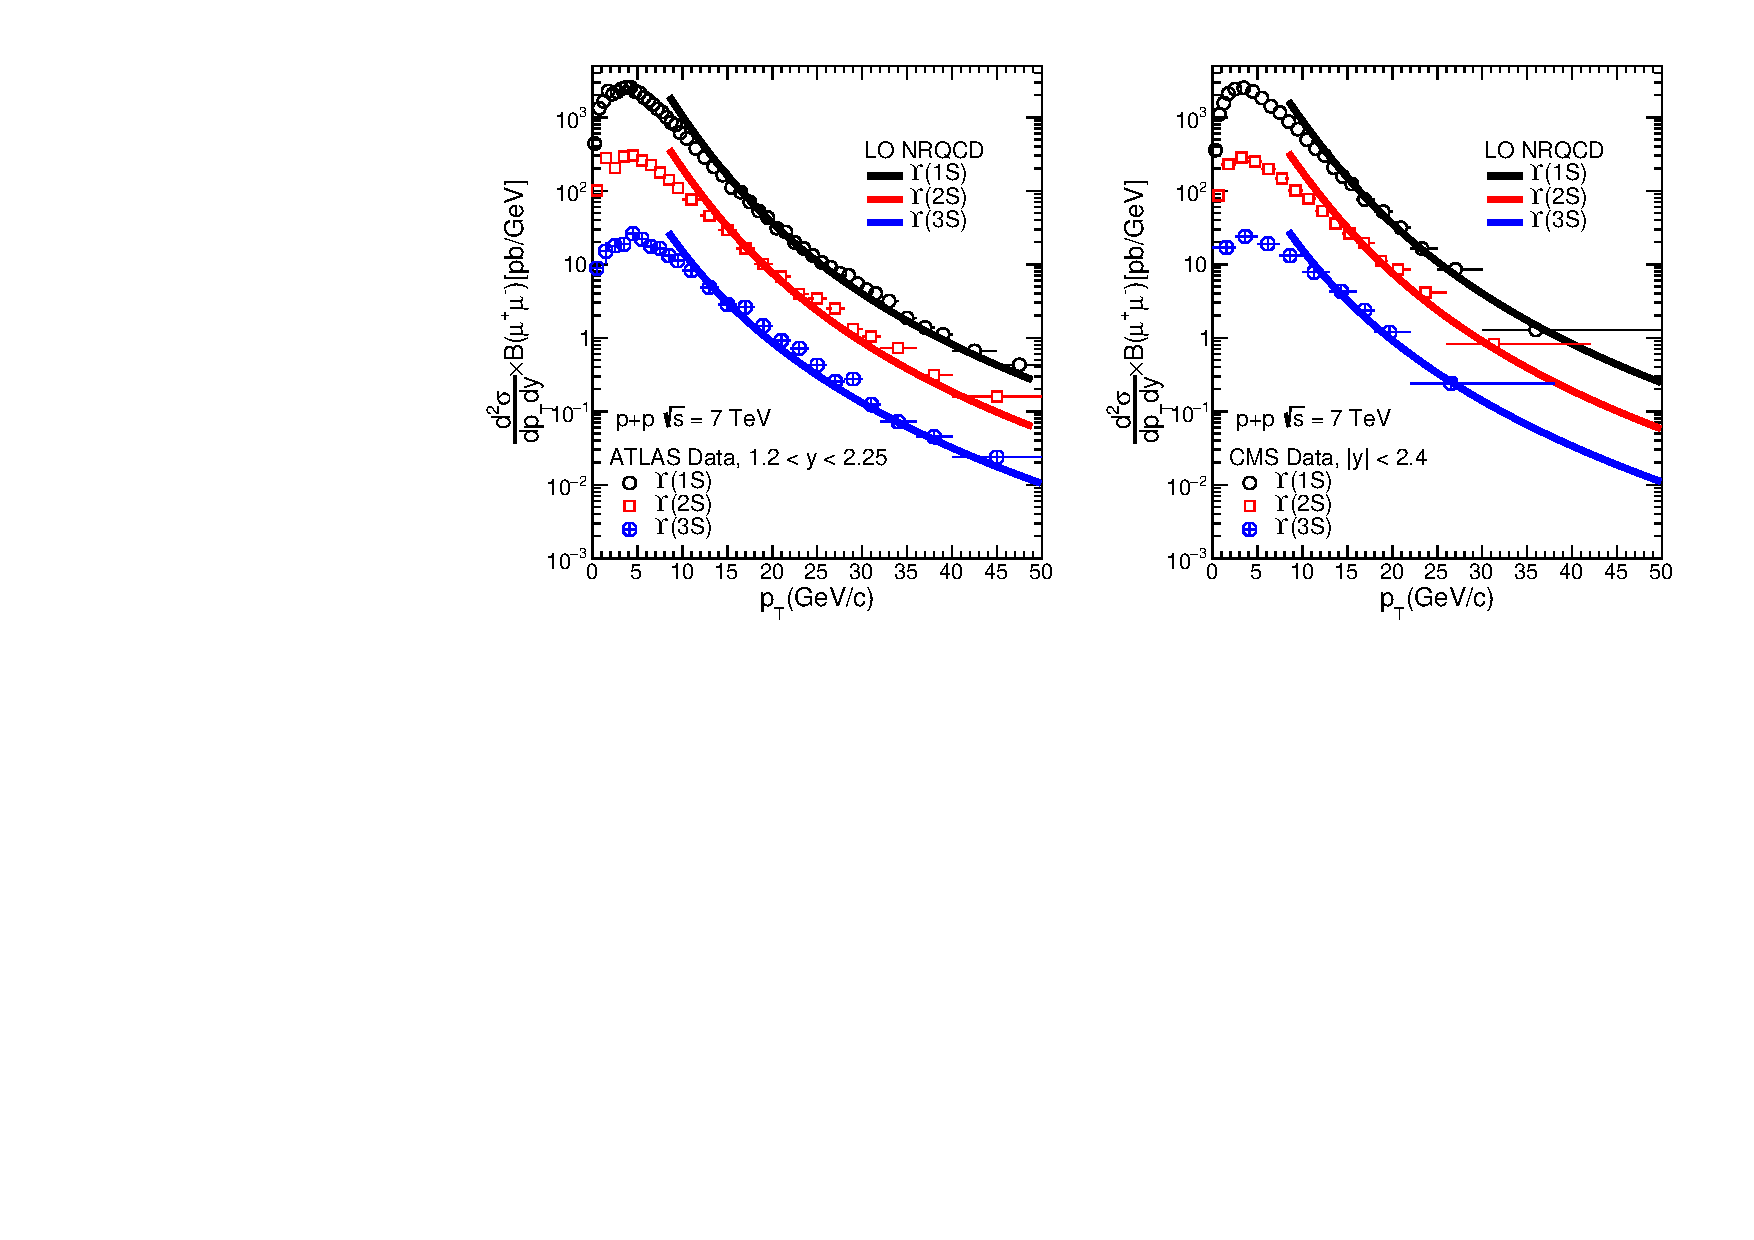
\includegraphics[width=0.99\textwidth]{Figures/NRQCD_Beauty/Fig_CMS_ATLAS_YnS_7TeV_Pt.pdf}
  \caption{\small{The NRQCD calculations~\cite{Kumar:2021sek} of production cross-section of $\Upsilon$(nS) in
      p+p collisions at $\sqrt{s}$ = 7 TeV, as a function of transverse momentum compared with
      the measured data by ATLAS~\cite{Aad:2012dlq} in left figure and CMS~\cite{Chatrchyan:2013yna}
      in right figure. The cross-section of $\Upsilon$(1S) and $\Upsilon$(2S) as well as
      calculations are shifted vertically by a constant factor for better visibility.}}
  %   The LDMEs are obtained by a combined fit of the CMS and ATLAS data.}
  \label{Fig:SigmaYnSCMS7TeV}
\end{figure}



The NRQCD formalism provides an adequate procedure to estimate a quantity as an expansion in 
heavy quark relative velocity, $v$ inside $Q\bar{Q}$ bound state. The LDME in Eq.(\ref{eq6})
do scale with definitive power in $v$. The quarkonium yield depends on the $^3S_1^{[1]}$ 
and $^3P_J^{[1]}$(J=0,1,2) CS states and $^1S_0^{[8]}$, $^3S_1^{[8]}$ and $^3P_J^{[8]}$
CO states in the limit $v\ll 1$.
%The quantity in the $[]$ stands for angular momentum
%quantum numbers of the meson in Fock expansion, whereas
The superscripts in square brackets represent the colour structure of the bound state,
1 for the CS and 8 for the CO.


%It is assumed that there is no significant feed down effect in $\Upsilon$(3S) from
%higher mass states like $\chi_{bJ}$(3P).

%\begin{figure}[!h]
%  \centering
%  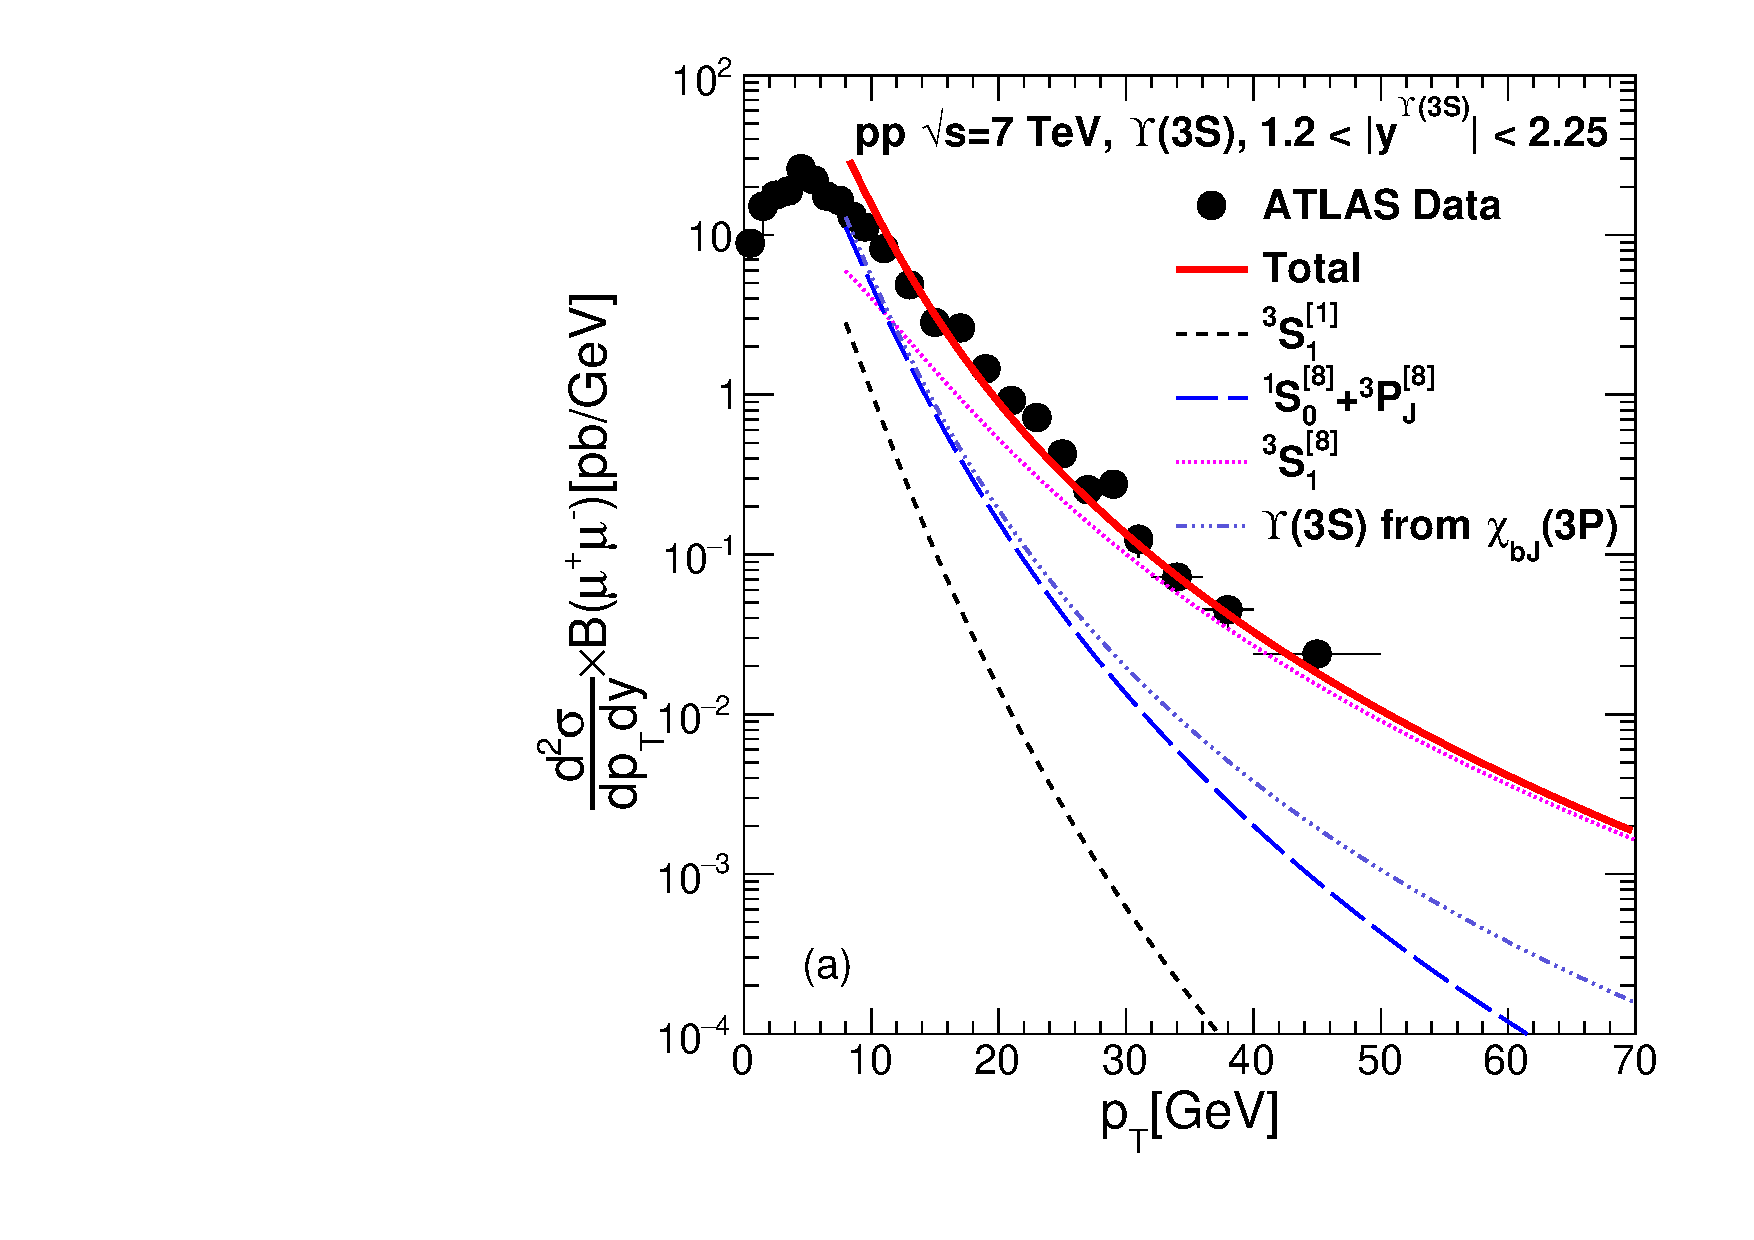
\includegraphics[width=0.49\textwidth]{Figures/NRQCD_Beauty/Fig2a_Y3S_ATLAS_Rap12225.pdf}
%  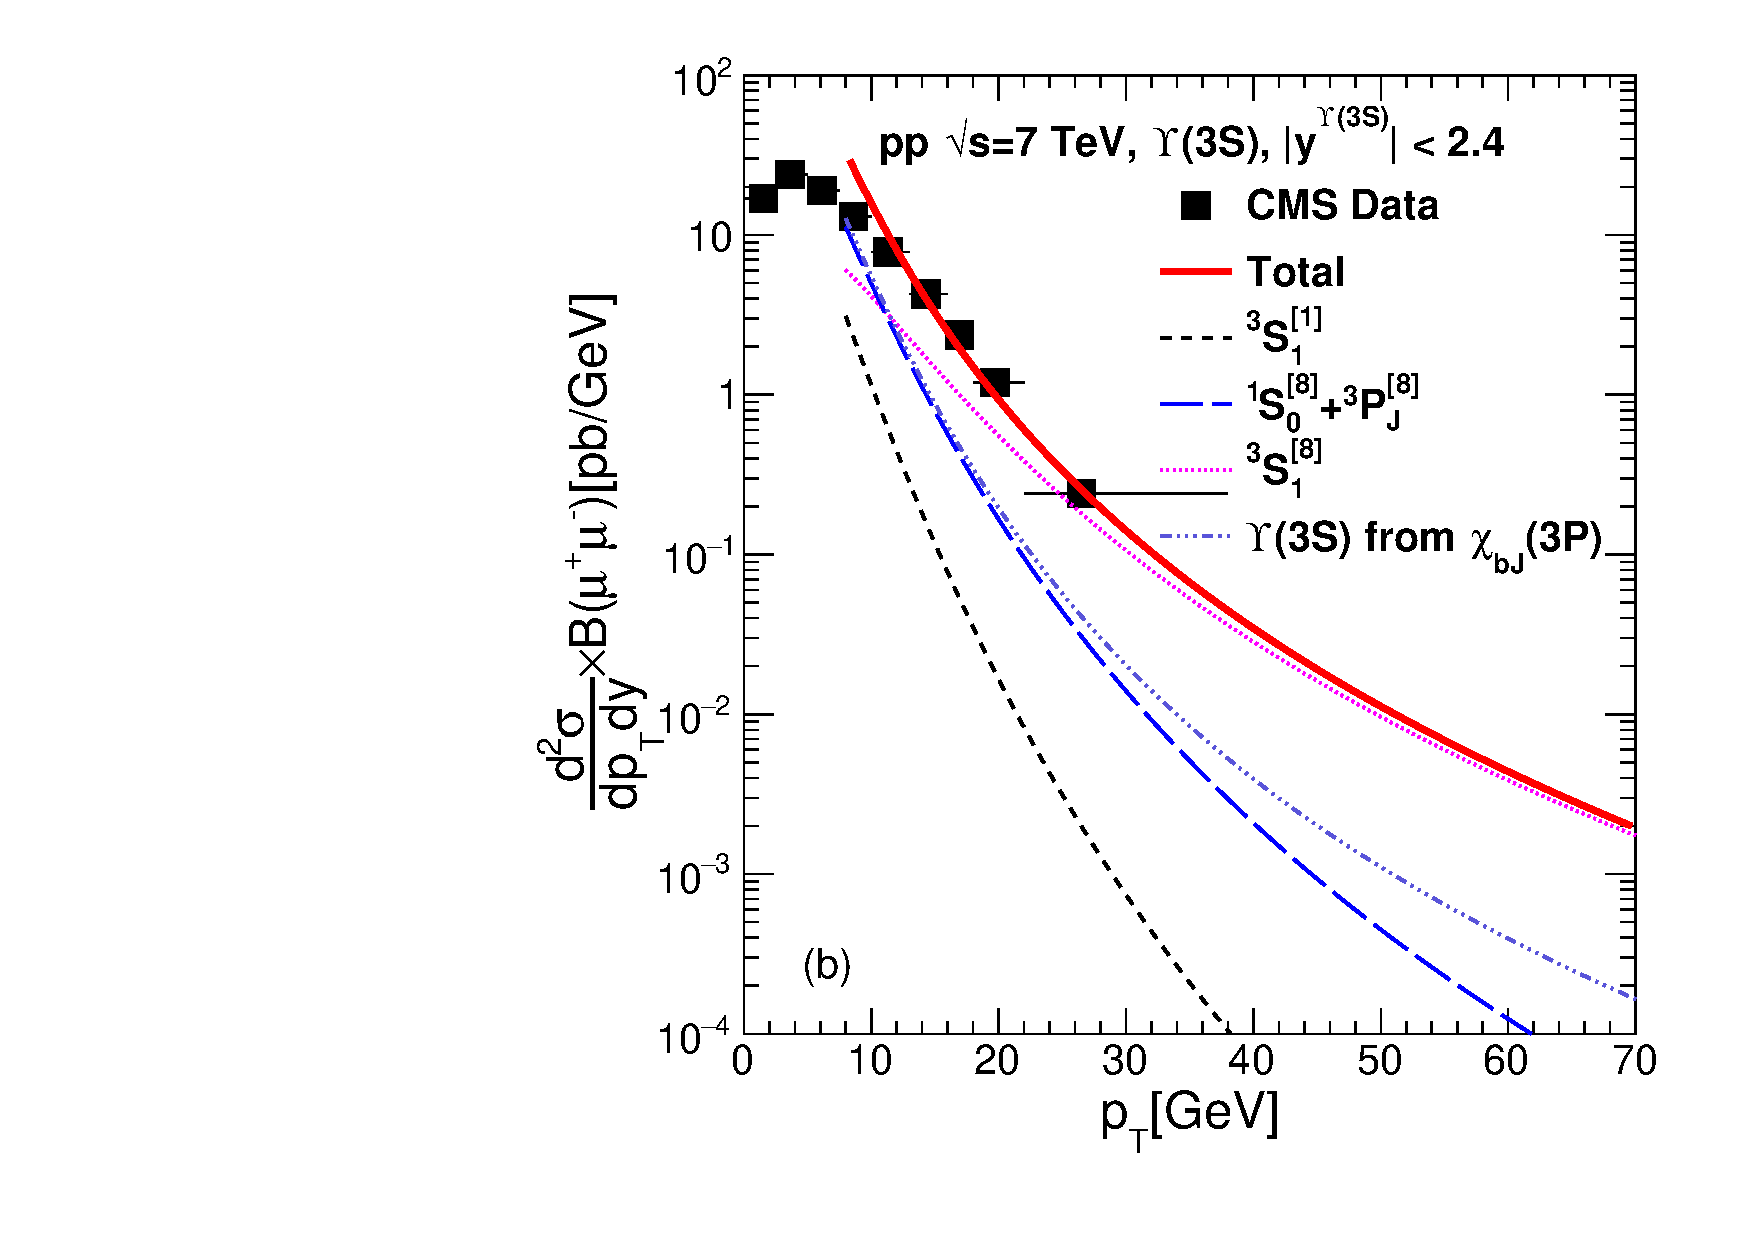
\includegraphics[width=0.49\textwidth]{Figures/NRQCD_Beauty/Fig2b_Y3S_CMS_Rapl24.pdf} 
%  \caption{\small{The NRQCD calculations of production cross-section of $\Upsilon$(3S) in p+p collisions at 
%      $\sqrt{s}$ = 7 TeV in forward rapidities, as a function of transverse momentum compared with the measured data 
%      at ATLAS~\cite{Aad:2012dlq} and CMS~\cite{Chatrchyan:2013yna} experiments. }}
%  %   The LDMEs are obtained by a combined fit of the CMS and ATLAS data.}
%  \label{Fig:SigmaY3SCMS_forwardRap}
%\end{figure}


One requires both CS and CO matrix elements in order to get theoretical
predictions for the production of bottomonia at the Tevatron and LHC energies.
The corresponding expressions and
numerical values for CS states are obtained from Ref.~\cite{Braaten:2000cm}.
The CO states, on the other hand, cannot be directly connected to the non-relativistic
wavefunctions of heavy mesons,
as these are associated with a higher Fock state. Experimentally measured data sets are 
therefore employed to obtain them as in Refs.~\cite{Braaten:2000cm,Cho:1995vh,Cho:1995ce}. 
%The CS operators along with their theoretical values
%and the CO operators to be fitted are listed in Table~\ref{CSCO},
%where, $n$=1,2,3.
For the CO elements related to p-wave states, needed as the 
feed down contributions, are obtained by Ref.~\cite{Sharma:2012dy,Feng:2015wka}.

Here we present the NRQCD results obtained in Ref.~\cite{Kumar:2021sek}.
The calculations use CT18NLO parametrisation~\cite{Hou:2019efy} for parton distribution
functions and the bottom quark mass $m_b$ is taken to be 4.88 GeV.
Measured transverse momentum distributions of $\Upsilon$(3S), 
$\Upsilon$(2S) and $\Upsilon$(1S) in p +{$\bar {\rm p}$} collisions at
$\sqrt{s}=$ 1.8 TeV and in p+p collisions at 7 TeV and 13 TeV are used to constrain
the LDMEs.

\begin{table*}
  \centering
  \caption{Comparison of CS elements and CO LDMEs extracted from fitting with experimental data
    using NRQCD formalism for $\Upsilon$(1S).}
  \footnotesize
  %\begin{tabular}{ccccccc}
  \begin{tabular*}{\textwidth}{@{\extracolsep{\fill}}lrrrrrl@{}}
    \hline
    \hline
    %& & & & & & \\
    Ref. (LO/NLO) & PDF & $m_b$ & $M_L(b\bar{b}([^3S_1]_1$ & $M_L(b\bar{b}([^3S_1]_8$ & 
    $M_L(b\bar{b}([^1S_0]_8$, & $p_T$-cut \\
    & & & $\rightarrow\Upsilon(1S)$ & $\rightarrow\Upsilon(1S)$ & $[^3P_0]_8\rightarrow\Upsilon(1S)$ & \\
    & & (GeV) & $({\rm GeV^3})$ & $({\rm GeV^3})$ & $({\rm GeV^3})$ & GeV/$c$ \\
    %& & & & & & \\
    \hline
    \hline
    & & & & & & \\
    \cite{Kumar:2021sek} (LO) & CT18 &4.88 &10.9 &0.0601$\pm$0.0017 & 0.0647$\pm$0.0016 & 8   \\
    %& (LO) & & & & & \\
    %\hline
    & & & & & & \\
    \cite{Domenech:2000ri} (LO) & CTEQ4L & 4.88 & 11.1 & 0.077$\pm$0.017 & 0 & 2 \\
    & & & & 0.087$\pm$0.016 & 0 & 4 \\
    & & & & 0.106$\pm$0.013 & 0 & 8 \\
    & & & & & & \\
    %\hline
    %& & & & & & \\
    \cite{Braaten:2000cm} (LO) & CTEQ5L & 4.77 & 12.8$\pm$1.6 & 0.116$\pm$0.027 & 0.109$\pm$0.062 & 8 \\
    & & & & 0.124$\pm$0.025 & 0.111$\pm$0.065 & \\
    & & & & & & \\
    & MRSTLO & 4.77 & 12.8$\pm$1.6 & 0.117$\pm$0.030 & 0.181$\pm$0.072 & 8 \\
    & & & & 0.130$\pm$0.028 & 0.186$\pm$0.075 & \\
    & & & & & & \\
    %\hline
    %& & & & & & \\
    \cite{Sharma:2012dy} (LO) & MSTW08LO & 4.88 & 10.9 & 0.0477$\pm$0.0334 & 0.0121$\pm$0.0400 & -  \\
    %& (LO) & & & & & \\
    %\hline
    & & & & & & \\
    \cite{Gong:2013qka} (NLO) & CTEQ6M & 4.75 & 9.282 & -0.0041$\pm$0.0024 & 0.0780$\pm$0.0043 & 8 \\
    %& (NLO) & & & & & \\
    %\hline
    & & & & & & \\
    \cite{Feng:2015wka} (NLO) & CTEQ6M & PDG & 9.282 & 0.0061$\pm$0.0024 & 0.0895$\pm$0.0248 & 8 \\
    %& (NLO) & & & & & \\
    \hline
    \hline
  \end{tabular*}
  \label{LDMEsY1S}
\end{table*}
%\normalsize

Figure~\ref{Fig:SigmaYnSCMS13TeV} shows the NRQCD calculations of production cross-section of $\Upsilon$(nS)
      in p+p collisions at $\sqrt{s}$ = 13 TeV in central rapidities, as a function of
      transverse momentum compared with the measured data at CMS~\cite{Sirunyan:2017qdw}
      experiment. The left figure shows relative contributions in $\Upsilon$(1S) from
      singlet and octet states as well as from feeddown. The right figure shows the sum
      of all contributions for all the 3 states where the results for $\Upsilon$(1S) and
      $\Upsilon$(2S) are shifted vertically by a constant factor for better visibility.


Figure~\ref{Fig:SigmaYnSCMS7TeV} shows the NRQCD calculations of production cross-section of $\Upsilon$(nS) in
      p+p collisions at $\sqrt{s}$ = 7 TeV, as a function of transverse momentum compared with
      the measured data by ATLAS~\cite{Aad:2012dlq} in left figure and CMS~\cite{Chatrchyan:2013yna}
      in right figure. The cross-section of $\Upsilon$(1S) and $\Upsilon$(2S) as well as
      calculations are shifted vertically by a constant factor for better visibility.

      The calculations for  $\Upsilon$(3S), $\Upsilon$(2S) and $\Upsilon$(1S) are compared with 
the measured data at Tevatron and LHC. The NRQCD formalism provides  very good description of the data in 
large transverse momentum range at different collision energy. 
   At high $p_T$, the colour singlet contribution is very small and LHC data in large $p_T$ range 
 help to constrain the relative contributions of different colour octet contributions.
  
Table~\ref{LDMEsY1S} shows the LDME values for $\Upsilon$(1S) obtained by 
different groups.







\subsubsection{Other methods}

In this section we, very briefly, touch upon two other processes namely
i) Fragmentation and ii) $k_T$ factorisation. 

\paragraph{Fragmentation}

In heavy ion collissions, partons with very high transverse momentum are produced.
When such a parton  with large transverse momentum $(k_T)$ decays into the final
hadronic state (quarkonium state here)~\cite{frag} then the process of production is called
fragmentation. At large enough $k_T$, quarkonium production is dominated by
fragmentation instead of the short distance mechanism which 
is suppressed by powers of $m_Q/k_T$ even though fragmentation is of higher
order in $\alpha_s$~\cite{frag}. 
 It was first shown by Braaten and Yuan~\cite{frag,frag1} that fragmentation of gluons and heavy quarks
 could be an important source of large-$k_T$ quarkonia production.
 There is a factorisation involved in the computation of the contribution 
 from the fragmentation process. A process like $A  B \rightarrow Q  X$ (where $A,B$ are  hadrons)
 is factorised  into a part containing the hard-scattering cross-section which produces
 a gluon or a heavy quark 
and a part which takes care of the fragmentation of the gluon or the heavy quark into the
relevant quarkonia state. One may write 
\begin{equation}
d\sigma (A  B \rightarrow Q X) = \sum_i \int_0^1 dz \ d\sigma  (A  B \rightarrow i  X) \ D_{i \rightarrow Q} (x,\mu)
\end{equation}
In the above equation $i$ is either a gluon or a heavy quark. The term $D_{i \rightarrow Q} (x,\mu)$ 
is called the fragmentation function which depends on the fraction of momentum of the parent parton 
carried by the quarkonia state $(x)$ and the scale $\mu$ which is of the order of $k_T$. 

 %{\bf ii) $k_T$ factorisation}
\paragraph{$k_T$ factorisation}

Another approach to quarkonium production is the $k_T$ factorisation method~\cite{kt1,kt2}.
In the  standard collinear approach, it is assumed that the momentum of all partons is
in the same direction as the initial particle. So the  transverse momentum $(k_T)$ is
considered to be zero. On the other hand, at large energies, the transverse
momentum $(k_T)$ is not negligible at all. 
 
In the $k_T$ factorisation approach, the quarkonium cross section is factorised
into two parts,  a cross section ${\hat \sigma} (x, k_T, \mu)$ and a parton
density function $f(x, k_T, \mu)$, where both depend on the transverse
momentum $k_T$~\cite{kt3}.  The quarkonium cross section is given by 
 
\begin{eqnarray}
   \sigma &=& \sum_{i,j} \int \frac {dx_1}{x_1} \frac {dx_2}{x_2} \
            f_i (x_1, k_{T,1}^2, \mu) \  f_j (x_2, k_{T,2}^2, \mu) \nonumber \\
    && \times \ {\hat \sigma}_{i+j \rightarrow X} (k_{T,1}, k_{T,2}, x_1, x_2, s) \ dk^2_{T,1} \ dk^2_{T,2}
\end{eqnarray}
where $i$ and $j$ are initial partons, $X$ is the final state,
$F(x, k_T, \mu)$ is the parton density function giving the probability of finding a parton
with given $x, k_T$, and $\mu$ and ${\hat \sigma}_{i+j \rightarrow X}$ is the parton cross
section giving the probability that initial partons $i$ and $j$ will form final state $X$.
